\chapter{Technical Approach}
\label{ch:tec}

In this chapter, we will explain the technical means by which the objective of this thesis has been approached. Firstly, in section \ref{s:pre} we start talking about the basic elements that have been used during the development this work. In order to make the robot avoid obstacles with proximity data, obstacles need to be located with respect to the robots’ kinematic chain. That's why, in section \ref{ss:calibration} we briefly present a framework for automatic kinematic calibration that leverages an IMU to accurately estimate the pose (position and orientation) of skin units along the surface of a robot. The main section is section \ref{s:control}, where the methods for collision avoidance are presented.

\section{Required resources}
\label{s:pre}
Introductory paragraph. General presentation of the required resources.

\subsection{Robot platform}
\label{ss:panda}

The robot utilized for the development of the ideas presented in this work has been the Panda, manufactured by the company Franka Emika based in Munich, Germany. It is well known for its performance and usability as well as for its affordability, starting at 10,000\$.

The Franka Emika Panda (FEP) is equipped with 7 revolute joints, i.e. it has 7 degrees of freedom (DOF). Each of the revolute joints mounts a torque sensor. The total weight of FEP is around \SI{18}{\kilo\gram}. It can handle payloads of up to \SI{3}{\kilo\gram}.


\begin{figure}[H]
    \caption[FEP's kinematic chain]{
        FEP: Joints and dimensions \cite{FrankaEmikaPanda}.
    }
    \begin{center}
    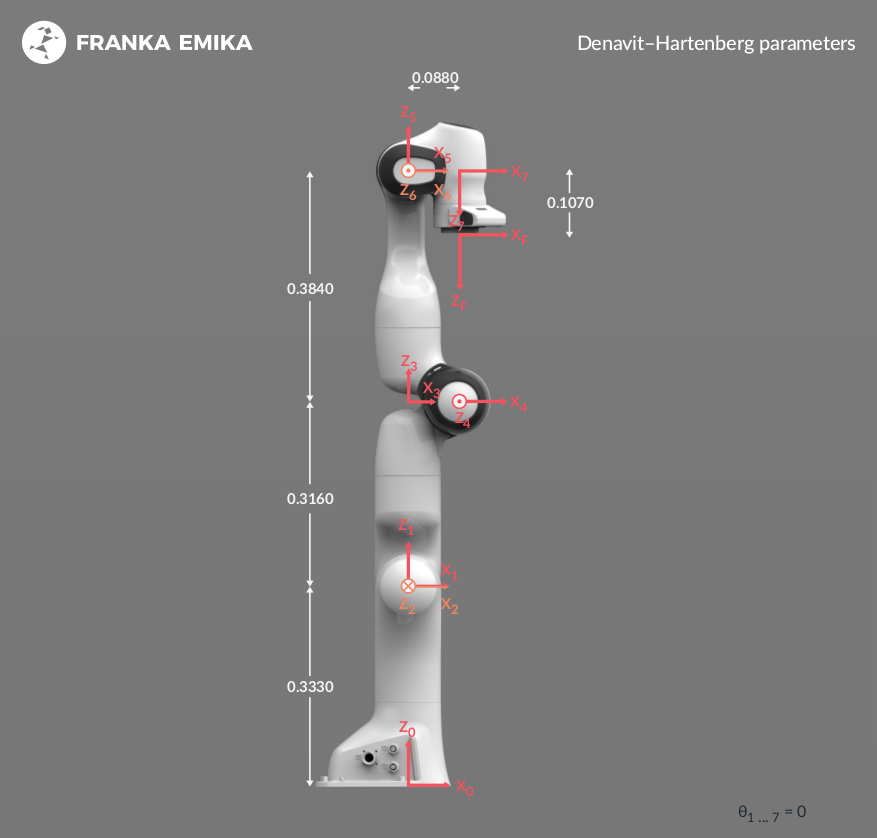
\includegraphics[width=\textwidth]{figs/panda-dh-diagram.png}
    \end{center}
\label{fig:FEPchain}
\end{figure}



It has a control interface that provides access to joint positions $\bf{q}$ and velocities $\dot{\bf{q}}$ and link side torques vector $\bf{\tau}$, with a refresh rate of \SI{1}{\kilo\hertz}. The control interface also provides numerical values of the inertia matrix \(\bar{\bf{M}}(\bf{q})\), the gravity vector \( \bar{\bf{g}}(\bf{q}) \), the end effector Jacobian matrix \( \bar{\bf{J}}(\bf{q}) \) and the Coriolis term \( \overline{\bf{c}}(\bf{q}, \dot{\bf{q}}) \).

There are 3 control modes available. At the lowest level, there is the torque-mode $\bf{\tau_d}$. The joint velocity $\dot{\bf{q_d}}$ and joint position $\bf{q_d}$ modes provide a higher level control and are the ones that are going to be used throughout this work.

The Denavit Hartenberg (DH) parameters provided by the manufacturer \cite{FrankaEmikaPanda} and depicted in figure \ref{fig:FEPchain} are shown in table \ref{t:dh}.

\begin{table}[H]
    \caption[Denavit Hartenberg parameters]{
        Denavit Hartenberg parameters \cite{FrankaEmikaPanda}
    }
    \begin{center}
    \begin{tabular}{|l|l|l|l|l|}
    \hline
        \textbf{Joint} & \textbf{a} (m) & \textbf{d} (m) & \(\mbox{\boldmath$\alpha$}\;(\text{rad})\) & \(\mbox{\boldmath$\theta$}\;(\text{rad})\) \\ \hline \hline
        1 & 0 & 0.333 & 0 & \(\theta_1\) \\ \hline
        2 & 0 & 0 & \(-\frac{\pi}{2}\) & \(\theta_2\) \\ \hline
        3 & 0 & 0.316 & \(\frac{\pi}{2}\) & \(\theta_3\) \\ \hline
        4 & 0.0825 & 0 & \(\frac{\pi}{2}\) & \(\theta_4\) \\ \hline
        5 & -0.0825 & 0.384 & \(-\frac{\pi}{2}\) & \(\theta_5\) \\ \hline
        6 & 0 & 0 & \(\frac{\pi}{2}\) & \(\theta_6\) \\ \hline
        7 & 0.088 & 0 & \(\frac{\pi}{2}\) & \(\theta_7\) \\ \hline
        F & 0 & 0.107 & 0 & 0 \\ \hline
    \end{tabular}
    \end{center}
\label{t:dh}
\end{table}

The manufacturer also provides the physical limits of the robot, both in the joint and the cartesian spaces (tables \ref{t:jointlimits} and \ref{t:cartesianlimits} respectively).

\begin{table}[H]
    \caption[Joint space limits]{
        Joint space limits \cite{FrankaEmikaPanda}
    }
    \begin{center}
    \begin{tabular}{|l|l|l|l|l|l|l|l|l|}
    \hline
         & Joint 1 & Joint 2 & Joint 3 & Joint 4 & Joint 5 & Joint 6 & Joint 7 & \\ \hline \hline
        \(\bf{q_{max}}\) & +2.8973 & +1.7628 & +2.8973 & -0.0698 & +2.8973 & +3.7525 & +2.8973 & \(\text{rad}\) \\ \hline
        \(\bf{q_{min}}\) & -2.8973 & -1.7628 & -2.8973 & -3.0718 & -2.8973 & -0.0175 & -2.8973 & \(\text{rad}\) \\ \hline
        \(\bf{\dot{q}_{max}}\) & 2.1750 & 2.1750 & 2.1750 & 2.1750 & 2.6100 & 2.6100 & 2.6100 & \(\frac{\text{rad}}{\text{s}}\) \\ \hline
        \(\bf{\ddot{q}_{max}}\) & 15 & 7.5 & 10 & 12.5 & 15 & 20 & 20 & \(\frac{\text{rad}}{\text{s}^2}\) \\ \hline
    \end{tabular}
\end{center}
\label{t:jointlimits}
\end{table}

\begin{table}[H]
    \caption[Cartesian space limits]{
        Cartesian space limits \cite{FrankaEmikaPanda}
    }
    \begin{center}
        \centering
        \begin{tabular}{|l|l|l|l|}
        \hline
             & \bf{Translation} & \bf{Rotation} & \bf{Elbow} \\ \hline \hline
            \(\bf{\dot{p}_{max}}\) & 1.7000 \(\frac{\text{m}}{\text{s}}\) & 2.5000 \(\frac{\text{rad}}{\text{s}}\) & 2.1750 \(\frac{rad}{\text{s}}\) \\ \hline
            \(\bf{\ddot{p}_{max}}\) & 13.0000 \(\frac{\text{m}}{\text{s}^2}\) & 25.0000 \(\frac{\text{rad}}{\text{s}^2}\) & 10.0000 \(\;\frac{rad}{\text{s}^2}\) \\ \hline
        \end{tabular}
    \end{center}
\label{t:cartesianlimits}
\end{table}

\subsection{ROS}
The Robot Operating System (ROS) is an open source robot middleware, robot framework or robot development environment (RDE), one of many available in the market. Robot middleware \cite{elkady2009middlew} is an abstraction layer that resides between the operating system (OS) and software applications (figure \ref{fig:middleware}). Its purpose is to provide a framework and  take care of several important parts of applications development, so that the developer needs only to build the logic or algorithm as a component.

\begin{figure}[H]
    \caption[Robotic middleware]{
        Robotic middleware \cite{elkady2009middlew}
    }
    \begin{center}
    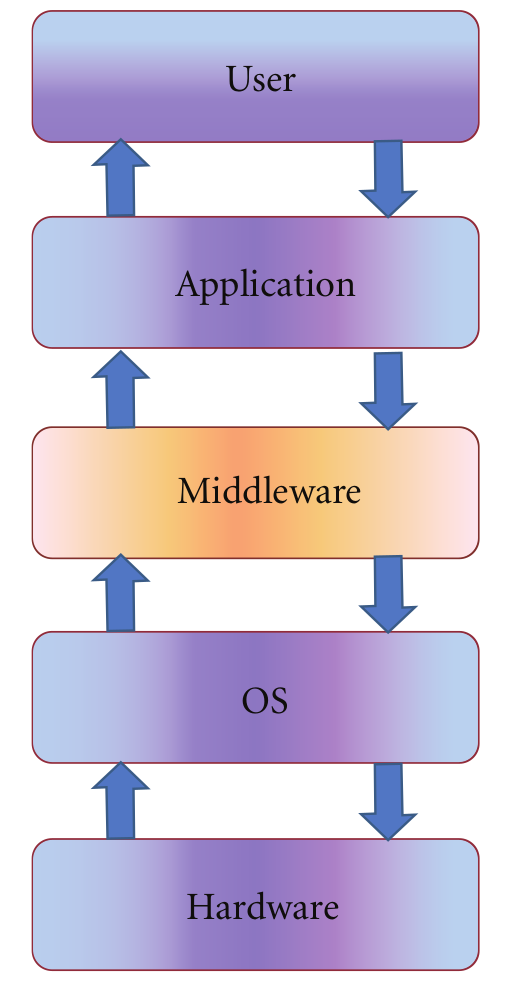
\includegraphics[width=45mm]{figs/middleware.png}
    \end{center}
\label{fig:middleware}
\end{figure}

The main goal of ROS in particular is to provide a framework for easy code reuse in research. This is why ROS is most extended in the academic context. It also provides APIs for Python and C++ and codes written in both languages can be used interchangeably and at the same time.

ROS’s main concept is its runtime graph: a peer-to-peer network of loosely coupled components or nodes that use the ROS communication infrastructure. ROS implements two main communication types:

\begin{itemize}
    \item\textbf{Topics.} A publisher node publishes a message to a topic. Another node subscribes to this topic, meaning that every time there is a new message published in the topic this subscriber node will receive it and therefore will we able to utilize and manipulate the data. Several nodes can publish to a given topic, as well as several nodes can also be subscribers of the same topic.
    \item\textbf{Services.} Sometimes the asynchronous model topics provide is not suitable. When synchronous behavior is desired services are the way to go. Services have two sides: client and service. From the client side calling a service is equivalent to calling a function. However, this function is managed in a different node: the server side.
\end{itemize}

In figure \ref{fig:rosgraph} the runtime graph of this work is presented as an example. The real robot is replaced by a simulation. The /gazebo node is calculating the physics of the real robot, as well as sensor readings.  /CartesianPositionController is subscribed to the topic /joint\_states, as it needs this information for control purposes. Sensor data is processed in the /proximity\_listener node and then is published to the topic /live\_points. This topic has two subscribers in these examples. On the one hand, /proximity\_visualizer uses the data published in /live\_points to visualize the sensor data in rviz (the 3D visualization tool provided by ROS to visualize several types of visual data). On the other hand,  /CartesianPositionController uses the data for collision avoidance control, as explained later in this chapter (section \ref{s:control}).

/robot\_state\_publisher is an example of the benefits of the framework ROS provides for easy code reuse. This node is part of a widely used ROS package that uses the robot’s description (described in a .urdf file) and messages published in /joint\_states to provide transformation matrices between any two joints in the robot’s kinematic chain. It publishes this data in /tf topics.

\begin{figure}[H]
    \caption[ROS graph]{
        ROS graph
    }
    \centering
    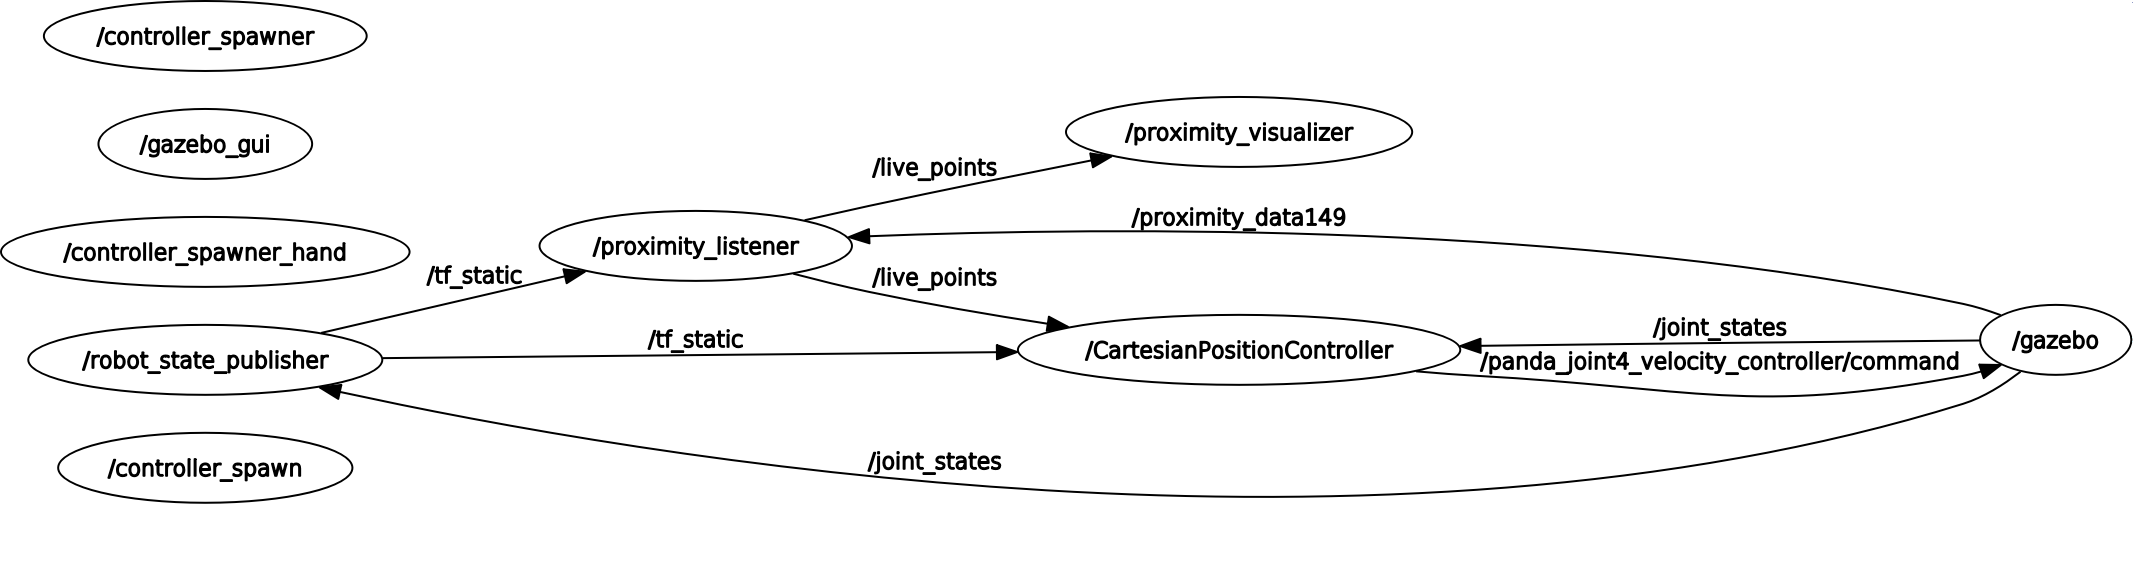
\includegraphics[width=\textwidth]{figs/rosgraph.png}
    \label{fig:rosgraph}
\end{figure}

In addition, bags in ROS enable real data storage coming from sensors in the robot. These allow developers to test their algorithms with real data without having to collect new data every time they need to run their code.

The ROS Master enables nodes to find each other and to communicate. It also holds the parameter server, which provides a central storage location for data that is relevant for several nodes. It serves, broadly speaking, as a place where global variables can be stored and retrieved by nodes. Examples of things that are stored in the parameter server are PID control parameters, the robot’s urdf description and frequencies at which different components living in the graph work.

Last, it should be mentioned that despite the fact that ROS is widely used in the academic context, it is lacking the reliability and robustness safety-critical systems in industrial or commercial contexts require. Some of the industrial fields, such as the automotive and the aerospace, have their own standards for the development of safety-critical software. These standards need to be certified for every software component written in any of these fields. ROS was not developed to any of these standards and it actually depends on many libraries that were not developed to these standards. ROS 2, in contrast, is based on components that are safety-certified (DDL communication) that make ROS 2 certifiable. Indeed, Apex.AI is working on Apex.OS: an API compatible to ROS 2 that is being certified ISO 26262 for safe automotive applications \cite{apexOS}.


\subsection{Simulation and Visualization}

According to the Cambridge Dictionary, a simulation is a situation in which a particular set of conditions is created artificially in order to study or experience something that could exist in reality. Simulations are therefore very useful for research and especially for robotics, where the following issues are prevalent:

\begin{itemize}
    \item Robotic hardware is usually \textbf{costy}.
    \item Prototyping can be \textbf{dangerous}, since bugs that appear when testing and debugging can lead to damage in the real world, as opposed to programs that only affect the virtual world.
    \item Development can be \textbf{slow}.
\end{itemize}

Robot simulation is a very addecuate solution to address each of these. This work has been prototyped in simulation. This has enabled parallel development of the artificial skin and its electronics on the one side and the control design on the other. The simulation software package employed has been \textit{Gazebo}.

\textit{Gazebo} \cite{gazebo} is a 3D robot simulator. It features dynamics simulation,  advanced 3D graphics, indoor and outdoor environments and simulation of several sensors with noise that make the virtual readings realistic. It is a standalone software package, but offers integration with ROS through the \textit{gazebo\_ros\_pkgs} ROS packages.

\begin{figure}[H]
    \caption[Gazebo]{
        Franka Panda Emika in Gazebo's simulation environment.
    }
    \centering
    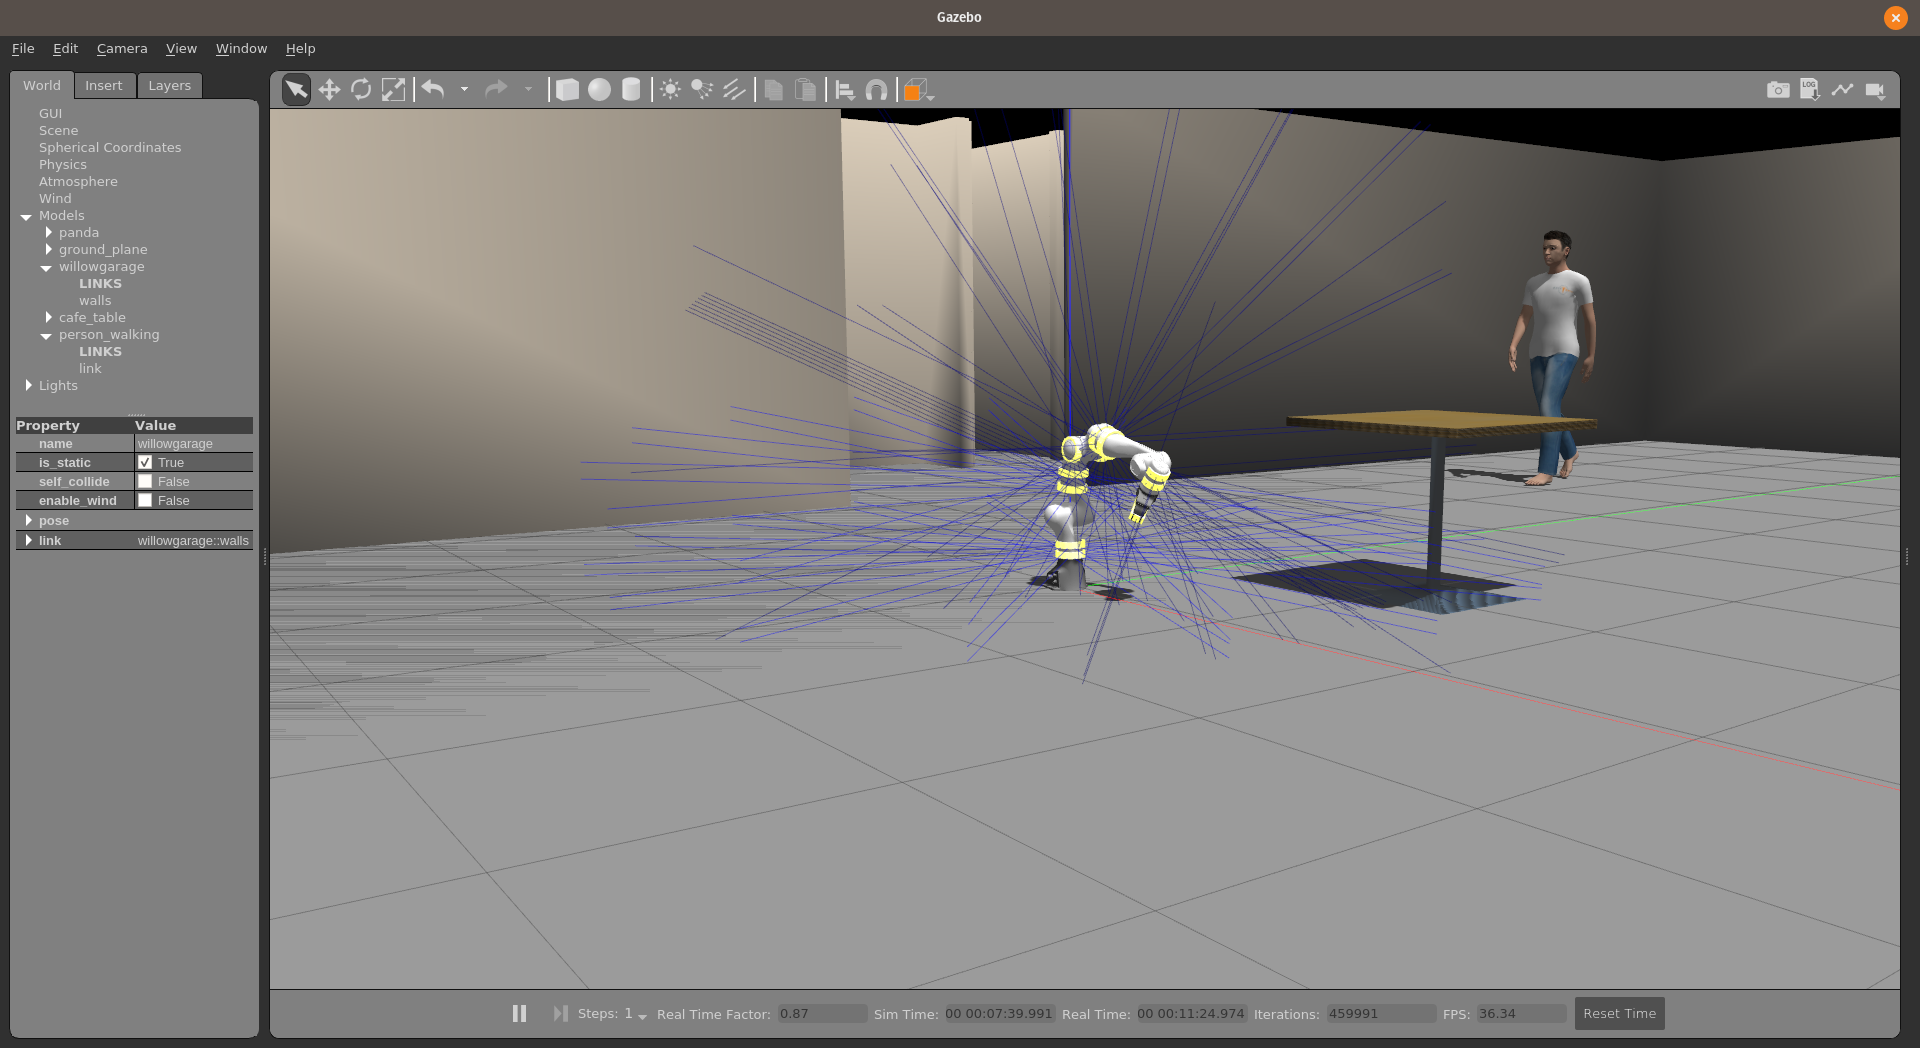
\includegraphics[width=\textwidth]{figs/gazebo_intro.png}
\end{figure}

On the other hand, ROS offers a useful vizualization tool called \textit{rviz} \cite{rviz}, short for \textit{ROS Visualization}. Several kinds of data can be visualized in \textit{rviz}, which allow to see what the robot is seeing, thinking and planning. These visualization capabilities make it an extremely useful tool for application debugging.

The difference between \textit{Gazebo} and \textit{rviz} is that even though both offer some kind of a graphics visualization, \textit{Gazebo} is mainly focused on simulating the physics whereas \textit{rviz} is mainly useful for visualizing any kind of information concerning the robot's state and its knowledge about the environment. Note that \textit{rviz} has the same role in both real and simulated environments.

\begin{figure}[H]
    \caption[rviz]{
        Joint frames in Franka Panda Emika as seen in \textit{rviz}.
    }
    \centering
    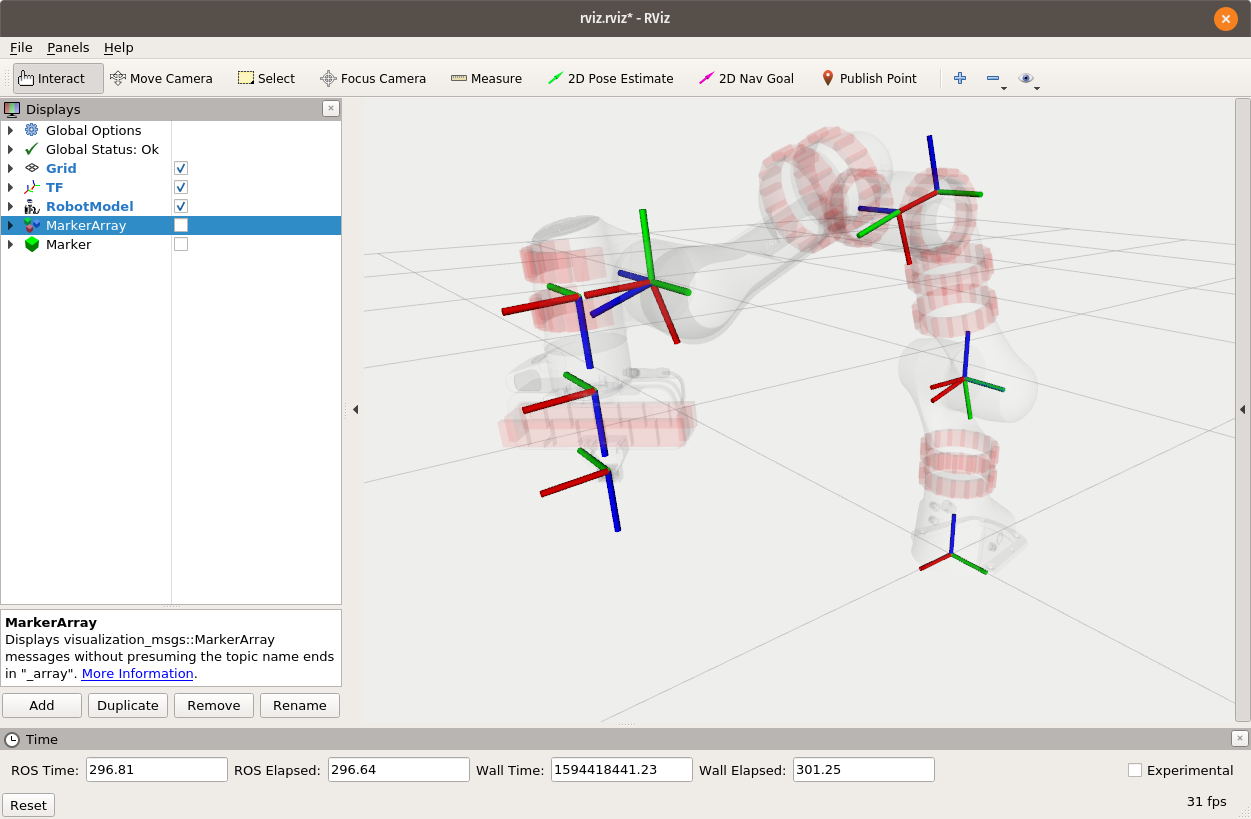
\includegraphics[width=\textwidth]{figs/rviz_intro.png}
\end{figure}



\subsection{Software Libraries}

In this section we describe the software libraries chosen to fulfill the needs that have arised during the implementation of the perception and control parts of this work. \textit{C++} is the language in which all the final code is written, so the libraries mentioned in this section are \textit{C++ Libraries}. Other languages (\textit{Python} and \textit{Matlab}) have also been employed in the code prototyping phase, but as their importance is less prevalent the software components employed in those languages will be mentioned in the specific parts they have been used, in section \ref{s:control}.

\subsubsection{Robot Kinematics}
\label{sss:KDL}

\textit{The Kinematics and Dynamics Library (KDL)} \cite{KDL} is a framework that provides the tools to describe robot kinematic chains and solutions to the most usual problems: forward and inverse kinematics, jacobian solvers, etc.

For that purpose, \textit{KDL} implements classes that represent kinematic primitives such as vectors, rotations and frames as well as classes that represent the whole kinematic chain, built from segments defined by kinematic primitives. The classes that represent the whole kinematic chain are \textit{KDL::Chain} and \textit{KDL::Tree}, being \textit{KDL::Tree} a container of \textit{KDL::Chain}s. Various generic forward and inverse kinematic algorithms that take objects of these classes are provided also.

For more information on the elements mentioned in this section see section \ref{ss:kinematiccontrol}, where the fundamental elements for basic kinematic control are discussed.

\subsubsection{Linear Algebra}

\textit{Eigen} \cite{eigen} is a \textit{template library} for linear algebra, meaning that every component in the Eigen is a \textit{C++ template}, that is, a component whose functionality can be adapted to more than one \textit{C++} type. In this case, Eigen supports all the \textit{C++} standard numeric types. It is the ecosystem of \textit{KDL} (\ref{sss:KDL}).

It supports fixed and dynamicly sized matrices and vectors and all the basic operations and common matrix decompositions. It does all its operations in an efficient, optimized, elegant and reliable fashion.

\subsubsection{Optimization}

ALGLIB \cite{alglib} is a numerical analysis and data processing library, which includes optimization algorithms among other tools. Its goal is to make high quality numerical code available to industry and academic worlds. The library is offered in a free version and in a commercial paid version, which is highly optimized. The free version, however offers access to the full library and has proved a good enough performance for this work.

\section{Perception via proximity sensing}
\label{s:perception}

Proximity sensors embedded in the artificial skin provide distance information about the surroundings of the robot. These readings are one dimensional distance readings, which means that the readings of isolated individual sensors are not very useful if our objetive is to obtain information about the 3D euclidean space in which the robot's operations take place.

In this section we describe the method developed in this work to create a 3D point cloud from proximity distance data. The first step is the kinematic calibration of the skin units that contain the proximity sensors. Kinematic calibration makes an automatic estimation of the position and orientation of each sensor. The method is described in section \ref{ss:calibration}. It is a conceptual and not detailed description, since it has been developed in a parallel project and is an essential part that make the control methods employed in this work possible. Section \ref{ss:pointcloud} describes the point cloud creation algorithm. Finally, section \ref{ss:visualization} shows how the obtained data is visualized in \textit{rviz}.

\subsection{Kinematic Calibration}
\label{ss:calibration}

This section describes a framework for automatic kinematic calibration that leverages an
\textit{Inertial Measurement Unit (IMU)} sensor to accurately estimate the position and orientation of a skin unit (SU) along the surface of a robot.

To automatically locate skin units along the surface of a robot, angular velocity and linear acceleration measurements from the IMUs are used. The position and orientation of an SU are estimated
using a modified version of \textit{Denavit-Hartenberg (DH) parameters} (see section \ref{sss:geomrep}), as illustrated in figure \ref{fig:calibration_theory}.
The position and orientation of each SU with respect to the previous
joint in the kinematic chain is estimated by six DH parameters: four parameters from the joint to a virtual joint,
and two additional parameters from the virtual joint to the SU (the other two parameters are set to $0$). This virtual joint is located within the link that is orthogonal to the joint’s $z$ axis and the SU’s $z$ axis.
This solution is necessary to adhere to the \textit{DH} notation,
so that each transformation can be expressed with no more than four parameters.

\begin{figure}[H]
    \caption[Calibration theory]{
        Depiction of multiple skin units (S) placed on the robots links (L) and separated by joints (J).
        We estimate the Denavit-Hartenberg parameters of each joint in order to calculate the pose of each skin unit along the surface of the robot.
    }
    \centering
    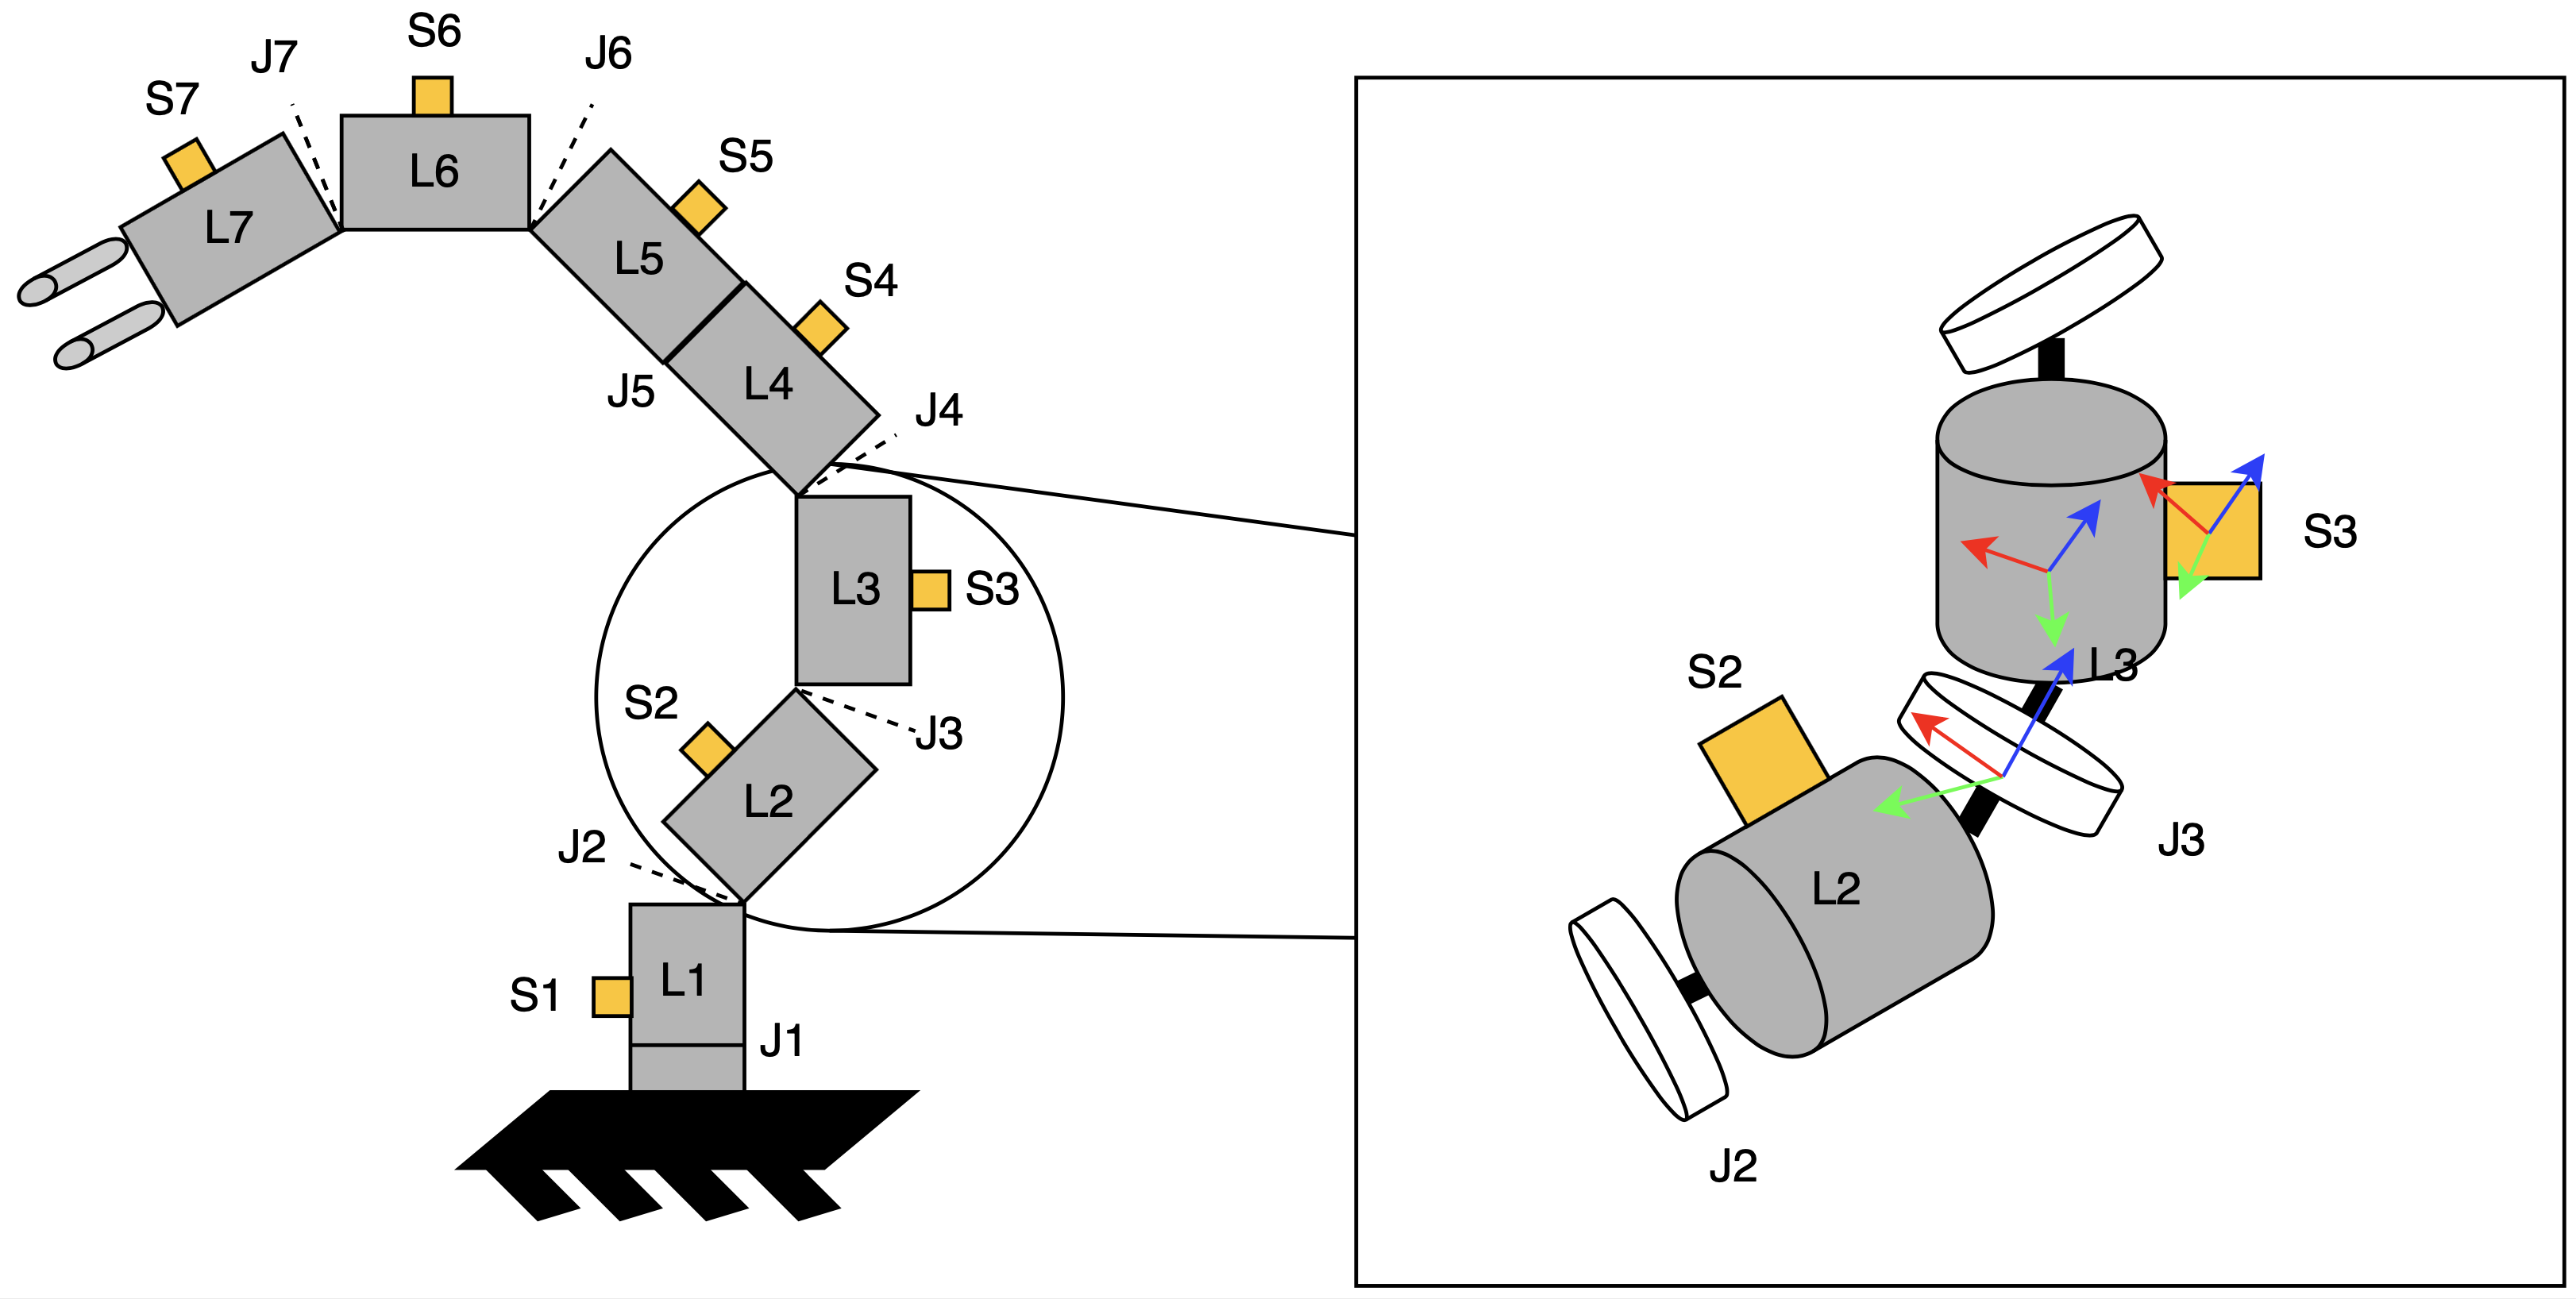
\includegraphics[width=\textwidth]{figs/calibration_theory.png}
\label{fig:calibration_theory}
\end{figure}

The optimization algorithm is composed of the following \textbf{four steps}:

\begin{enumerate}
    \item \paragraph{Initialize a kinematic chain with randomized values.}
    Each skin unit frame is represented using an homogeneous transformation matrix (see section \ref{sss:FK}).
    $${}^0T_{SU_i} = {}^0T_1 \cdot {}^1T_2 \dots {}^{i-1}T_i \cdot {}^i T_{SU_i}, \quad \forall i \in \{1,2, \dots, n\}$$

    \item \paragraph{Collect Data.}
    First, static forces applied to the IMU (that is, the constant acceleration due to gravity)
    are measured and compensated for.
    Then, each reference joint is moved through its operational range in a constant rotation pattern
    and the resulting acceleration as measured by the IMU is stored.

    \item \paragraph{Define an error function.}
    Acceleration exerted on each SU ${}^{SU_i}a_{u,d}$ can be estimated as a composition of local acceleration $^{0} \mathbf{g}$,
    tangential acceleration $^{0}\mathbf{a}_{t a n_{u, d}}$ and centripetal acceleration $^{0}\mathbf{a}_{cp_{u, d}}$:
    $$^{0}\mathbf{a}_{t a n_{u, d}} = ^{0}\bfgreek{\alpha}_{d} \times^{0} \mathbf{r}_{u, d}$$

    $$^{0}\mathbf{a}_{cp_{u, d}} = ^{0}\bfgreek{\omega}_{d} \times \left(^{0}\bfgreek{\omega}_{d} \times^{0} \mathbf{r}_{u, d}\right)$$

    $$^{SU_{i}}\mathbf{a}_{u, d} = ^{SU_{i}}\mathbf{R}_{0} \cdot\left(^{0} \mathbf{g}+^{0} \mathbf{a}_{t a n_{u}, d}+^{0} \mathbf{a}_{c p_{u, d}}\right).$$

    Angular velocity $^{0}\bfgreek{\omega}_{d}$ and angular acceleration $^{0}\bfgreek{\alpha}_{d}$ are measured during data collection, whereas rotation matrix $^{SU_{i}}\mathbf{R}_{0}$ and position vector $^{0} \mathbf{r}_{u, d}$ can be computed using the currently estimated DH parameters.

    \item \paragraph{Minimize the error function with a global optimizer.}
    A global optimizer optimizes the DH parameters by minimizing a given error function. One example error function could be seen as the error between the measured accelerations from the IMUs and the estimated accelerations using the kinematic chain model for $n_{pose}$ poses:
    $$E = \sum_{i=1}^{n_{pose}} \sum_{j=1}^{n_{joint}} ||a^{model}_{i,j} - a^{IMU}_{i,j}||^2$$

    Several different error functions are used to estimate both rotational and translational parameters.

\end{enumerate}

The final result after calibration can be seen in figure \ref{fig:calibration_result}.. Once the calibration is completed, the positions and orientation of the SU's are known. In the next section we will describe how 3D located points can be obtained from the positions and orientations of the sensors plus their readings.

\begin{figure}[H]
    \caption[Calibration result]{
    Calibrated IMU positions on a simulated Franka Emika Panda robot.
    }
    \begin{center}
    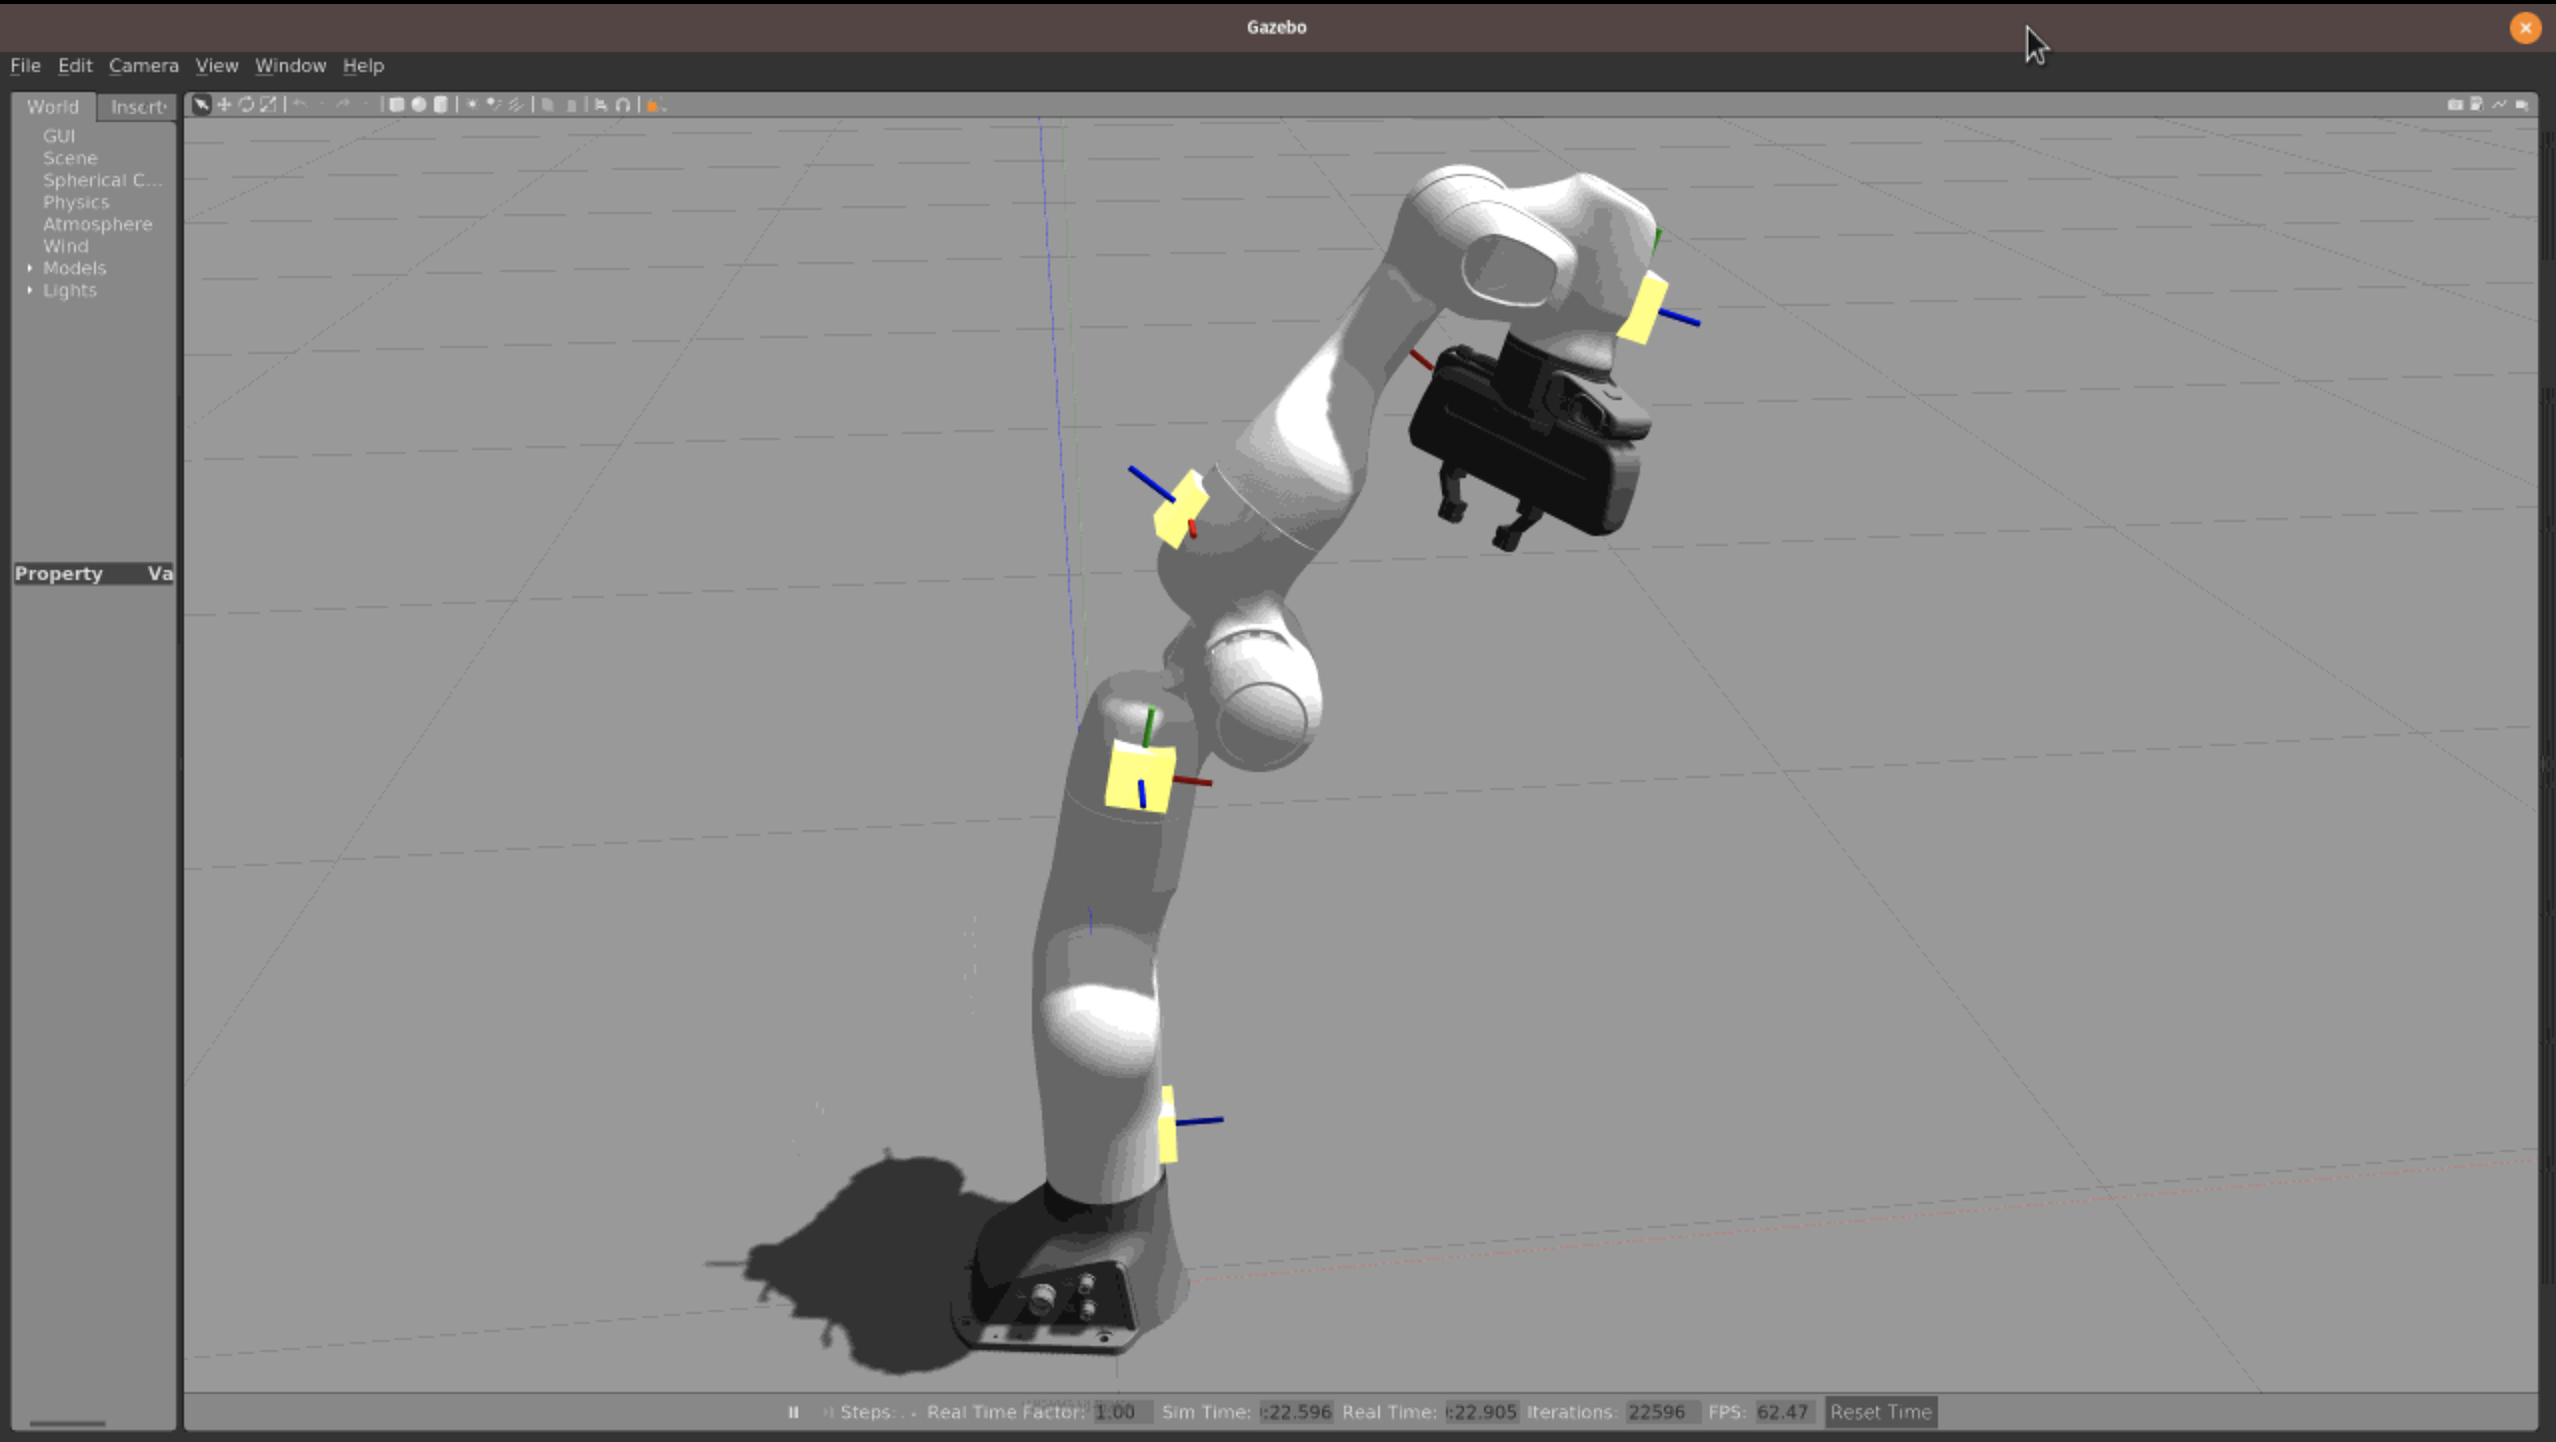
\includegraphics[width=\textwidth]{figs/calibration_result.png}
    \end{center}
\label{fig:calibration_result}
\end{figure}

\subsection{Simulation of proximity sensors}
\label{ss:proximitysimulation}

We start by describing the algorithm's implementation with simulated sensors. There are some important differences compared to using real sensors:

\begin{itemize}
    \item The sensors' positions and orientations are assumed to be known. A perfect outcome from calibration is assumed.
    \item The number of sensors that we can place on the robot's surface is unlimited.
    \item Sensor noise can be contolled.
\end{itemize}

In order to add proximity sensors to the robot suface in simulation \textit{XML macros (xacro)} are utilized. \textit{Xacro}'s allow to write shorter, easier to maintain and more readable XML files. One xacro macro expand into a larger XML expression. Moreover, it allows math, which is useful as we will see in the following lines.

We start by describing how to set up the behaviour of the proximity sensors in Gazebo. Gazebo provides the ability to add new functionalities to the \textit{urdf} models through the use of plugins. More specificly, it is sensor plugins that provide sensor simulation functionalities. Sensor plugins are inserted in the \textit{urdf} description of the robot model in \lstinline[columns=fixed]{<gazebo>} tags. Since the sensors are meant to be attached to a link, this tag must include a reference to indicate the link in which the sensor is inserted, as seen in line \ref{code:gazebotag} in the code below.

\begin{lstlisting}[caption={Setting up a ray sensor for Gazebo simulation.},captionpos=b]
<gazebo reference="proximity_link${proximity_id}"> (*\label{code:gazebotag}*)
    <material>Gazebo/YellowGlow</material>
    <sensor type="ray" name="proximity_sensor${proximity_id}">
        <pose>0 0 0 0 0 0</pose>
        <visualize>true</visualize>
        <update_rate>${freq}</update_rate>
        <ray>
            <scan>
                <horizontal>
                    <samples>1</samples>
                    <resolution>1</resolution>
                    <min_angle>-0.0001</min_angle>
                    <max_angle>0.0001</max_angle>
                </horizontal>
            </scan>
            <range>
                <min>0.02</min>
                <max>2.0</max>
                <resolution>0.01</resolution>
            </range>
        </ray>
        <plugin filename="libgazebo_ros_laser.so"
                name="proximity_plugin${proximity_id}">
            <topicName>proximity_data${proximity_id}</topicName>
            <bodyName>proximity_link${proximity_id}</bodyName>
            <updateRateHZ>${freq}</updateRateHZ>
            <gaussianNoise>0.0</gaussianNoise>
            <xyzOffset>0.0 0.0 0.0</xyzOffset>
            <rpyOffset>0 0 0</rpyOffset>
            <frameName>proximity_link${proximity_id}</frameName>
        </plugin>
    </sensor>
</gazebo>
\end{lstlisting}

Gazebo provides several sensor plugins \cite{gazeboplugins}, such as depth cameras, \textit{IMU}'s or force sensors. The proximity sensing capabilities are provided in \textit{laser} sensors. These are originally thought to simulate \textit{LIDAR} sensors, where a number of distance sensors are installed in one module. However, in order to simulate a single proximity sensor we only need an individual laser beam. The final configuration that accomplishes this is shown between in the \lstinline[columns=fixed]{<ray>} tag.

The sensor messages are published to the topic \lstinline[columns=fixed]{/proximity_data#} and the type of the messages published is \lstinline[columns=fixed]{sensor_msgs/LaserScan}, which is structured as follows:


\begin{lstlisting}[caption={LaserScan message structure.},captionpos=b, numbers=none]
    std_msgs/Header header
        uint32 seq
        time stamp
        string frame_id
    float32 angle_min
    float32 angle_max
    float32 angle_increment
    float32 time_increment
    float32 scan_time
    float32 range_min
    float32 range_max
    float32[] ranges
    float32[] intensities
\end{lstlisting}

Once we know how to set up the sensors, we need to place them in the robotic arm. Since the arms are mainly cylindrical, cylindrical coordinate systems $(r,\theta, z)$ are a more suitable solution to refer to points on the surface than regular cartesian $(x, y, z)$. \textit{urdf} only allows to express positions in $(x, y, z)$, but math provided by xacro can be utilized to express cylindrical coordinates in those required cartesian coordinates.

\begin{equation}
    \label{eq:cylindrical}
    \begin{split}
& x = r \cos \theta \\
& y = r \sin \theta \\
& z = z
    \end{split}
\end{equation}

Therefore, the proximity sensor macro allows to use cylindrical coordinates to create a new link attached to the surface of the robot that simulates a new proximity sensor. The interface to the macro is defined by the arguments it takes. These is a list of these arguments:

\begin{itemize}
    \item \textbf{proximity\_id}: It is important to define a unique name for the link and joint. Trying to use an already defined name will result in an error.
    \item \textbf{connected\_to}: It is used to select the link in which the sensor is placed. The link's coordinate frame's $z$ axis must be oriented in the direction of the arm cylinder. In other words, link's whose coordinate frames are not oriented in this way are not valid.
    \item \textbf{type}: It allows to specify the joint type: fixed, revolute or prismatic. In this case, it could have been previously set to fixed.
    \item \textbf{x0}, \textbf{y0}: If the $z$ axis is not centered in the desired cylinder \lstinline[columns=fixed]{x0} and \lstinline[columns=fixed]{y0} can apply an offset to place the origin where it is needed.
    \item \textbf{radius}, \textbf{theta}, \textbf{z0}: The cylindrical coordinates presented in equation \ref{eq:cylindrical}.
\end{itemize}

The actual implementation of the macro can be seen in the following fragment of a \textit{xacro} code. Cylindrical coordinates are implemented in the \lstinline[columns=fixed]{<origin>} tag at line \ref{code:cylindrical}.

\begin{lstlisting}[caption={$<$joint$>$ element in the proximity macro, where the position of new sensor is set up given some arguments.},captionpos=b]
<!-- Connect proximity sensor to ${connected_to} -->
<joint name="proximity${proximity_id}_to_${connected_to}"
        type="${type}">
    <parent link="${connected_to}"/>
    <child link="proximity_link${proximity_id}"/>
    <origin (*\label{code:cylindrical}*)
        xyz="${x0+radius*sin(theta)} ${y0+radius*cos(theta)} ${z0}"
        rpy="0 0 ${pi/2 -theta}" />
</joint>
\end{lstlisting}

We can use this macro to place sensors through a number of rings to cover the body of the robot and simulate the artificial skin. \lstinline[columns=fixed]{radius} specifies the selected link's radius and \lstinline[columns=fixed]{z0} decides de longitudinal position in with we want to place the sensor. With \lstinline[columns=fixed]{radius} and \lstinline[columns=fixed]{z0} fixed, changing \lstinline[columns=fixed]{theta} can place sensors through the entire ring \lstinline[columns=fixed]{radius} and \lstinline[columns=fixed]{z0} define. The following code places 4 equally spaced sensors in a ring located in panda link 3.

\begin{lstlisting}[caption={Using the proximity macro to place sensors in a robot arm.},captionpos=b]
<xacro:property name="sensors_per_ring" value="4"/>
<xacro:property name="ring_id" value="0"/>
<xacro:property name="radius" value="0.06"/>
<xacro:property name="z0" value="-0.13"/>
<xacro:property name="connected_to" value="panda_link3"/>
<xacro:proximity proximity_id="${sensors_per_ring*ring_id+0}"
                 radius="${radius}"
                 theta="${2*pi/sensors_per_ring* 0}"
                 z0="${z0}" connected_to="${connected_to}"/>
<xacro:proximity proximity_id="${sensors_per_ring*ring_id+1}"
                 radius="${radius}"
                 theta="${2*pi/sensors_per_ring* 1}"
                 z0="${z0}" connected_to="${connected_to}"/>
<xacro:proximity proximity_id="${sensors_per_ring*ring_id+2}"
                 radius="${radius}"
                 theta="${2*pi/sensors_per_ring* 2}"
                 z0="${z0}" connected_to="${connected_to}"/>
<xacro:proximity proximity_id="${sensors_per_ring*ring_id+3}"
                 radius="${radius}"
                 theta="${2*pi/sensors_per_ring* 3}"
                 z0="${z0}" connected_to="${connected_to}"/>
\end{lstlisting}

The final appearance of the new sensor links added to the surface of the robot is shown in figure \ref{fig:sensorssimulation}, where the new links are shown as red parallelepipeds. The final amount of sensors added for simulation counts $162$.

\begin{figure}[H]
    \caption[proximity sensors]{
    Robot body covered with proximity sensors, which appear in red.
    }
    \begin{center}
    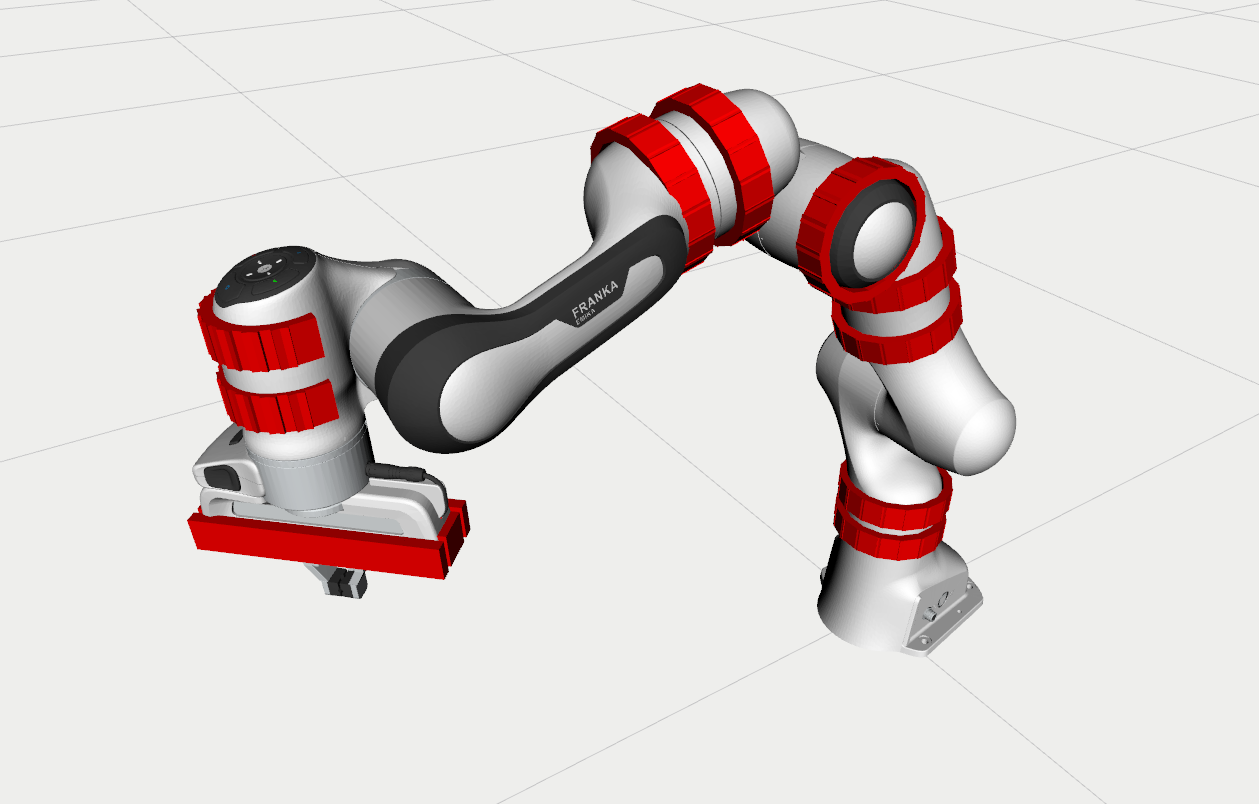
\includegraphics[width=\textwidth]{figs/sensors_simulation.png}
    \end{center}
\label{fig:sensorssimulation}
\end{figure}

\subsection{Point localization algorithm}
\label{ss:pointcloud}

The question answered in this section is: How do we convert the unidimensional reading of the proximity sensors embedded in the skin into a 3D point cloud in the cartesian space.

The diagram in figure \ref{fig:sensorreadingconversion} shows the relationship between the unidimensional reading $d_i$ and the position vector of the corresponding point with respect to the base frame $O$.

\begin{figure}[H]
    \caption[]{
    Diagram showing the conversion of a proximity sensor reading into a 3D point in space.
    }
    \begin{center}
    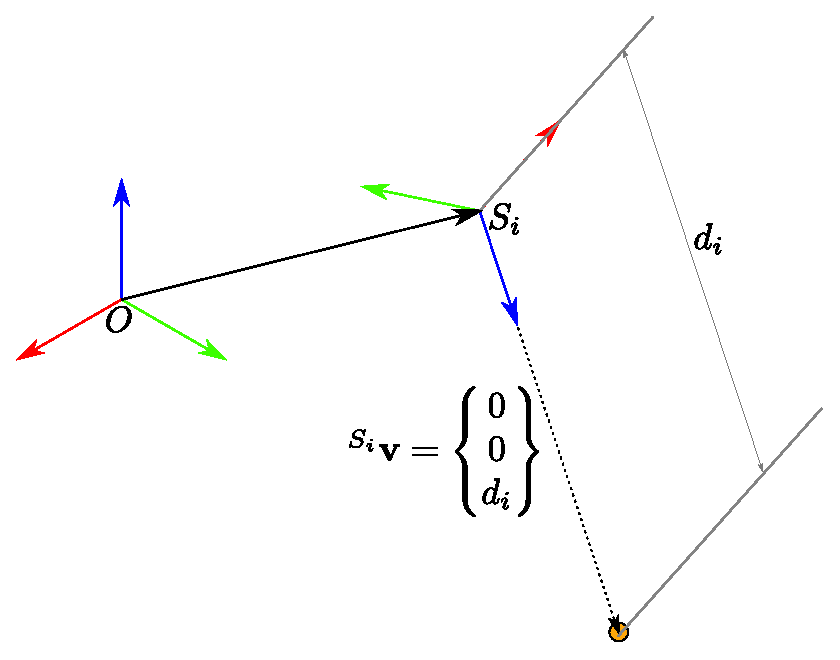
\includegraphics[width=100mm]{figs/proximity_sensors.eps}
    \end{center}
    \label{fig:sensorreadingconversion}
\end{figure}

The position of orientation $^{j}\mathbf{T}_{S_i}$ of the sensor $S_i$ with respect to the joint $j$ in which its located are obtained after the calibration process presented in section \ref{ss:calibration}. This allows to obtain the position and orientation $^{0}\mathbf{T}_{S_i}$ of the sensor $S_i$ with respect to the base frame $O$, through forward kinematics (explained in section \ref{sss:FK}).

$$
^{0}\mathbf{T}_{S_i} = ^{0}\mathbf{T}_{j} \cdot ^{j}\mathbf{T}_{S_i}
$$

Once $^{0}\mathbf{T}_{S_i}$ is known, the next step is calculating the position vector of obstacle associated to the sensor $S_i$ with respect to the base frame. The distance $d_i$ is read in the $z$ axis of $S_i$ (coloured in blue in the diagram in \ref{fig:sensorreadingconversion}). Therefore, the position of the point detected written in the $S_i$ coordinate frame has the following form:

$$
^{S_i}\mathbf{v} =
\begin{Bmatrix}
0\\
0\\
d_i
\end{Bmatrix}
$$

Again, simple forward kinematics allow us to transform that vector in order to express in in the base coordinate frame $O$.

$$
^{0}\mathbf{v} = ^{0}\mathbf{T}_{S_i} \: ^{S_i}\mathbf{v}
$$

Expanding the expression having into account the form of homogeneous transformation matrices, $^{0}\mathbf{v}$ results in:


\begin{equation}
\label{eq:livepoints}
^{0}\mathbf{v} = ^{0}\mathbf{p}_{S_i} + ^{0}\mathbf{R}_{S_i} \: ^{S_i}\mathbf{v}
\end{equation}

As stated in section \ref{ss:proximitysimulation}, each proximity sensor publishes a \lstinline{LaserScan} type message to the topic \lstinline{/proximity_data#}. We have implemented a \textit{ROS} node that deals with the transformations presented in this section when new messages are published to the topics and we have named it \lstinline{proximity_listener}. The node's activity can be summarized in $3$ steps:

\begin{enumerate}
    \item Listen to changes in the topics to which proximity sensors send data.
    \item Transform the unidimensional sensor readings into 3D position vectors.
    \item Publish the updated 3D position vectors with a certain periodicity. Also, allow saving old obstacle points for a while, so that a memory of the last reading is kept.
\end{enumerate}

In the following paragraphs we expand on these steps. First, the callback function is explained, where steps (1) and (2) are carried out. Then, the publication of messages and buffer implementation are detailed in step (3).

\textit{ROS} suscribers implement a callback function, which allows them to process the data published in the subscribed topics. This callback function is called every time a new message arrives to the topic. The callback that receives the proximity sensor data is presented below.

\begin{lstlisting}[caption={Point localization \textit{C++} algorithm.},captionpos=b]
void sensorCallback(const sensor_msgs::LaserScan::ConstPtr& scan)
{
int sensor_number = (*\label{code:readsensornumber}*)
    std::stoi
    (
        scan->header.frame_id.substr
        (
            scan->header.frame_id.find_first_of("0123456789"),
            scan->header.frame_id.length() -1
        )
    );

try
{
    listener.lookupTransform
    (
        "/world",
        "/proximity_link" + std::to_string(sensor_number),
        ros::Time(0),
        transform[sensor_number]
    );
    translation1[sensor_number] <<
        transform[sensor_number].getOrigin().getX(),
        transform[sensor_number].getOrigin().getY(),
        transform[sensor_number].getOrigin().getZ();
    translation2[sensor_number] << 0.0,
                                   0.0,
                                   scan->ranges[0];
    rotation[sensor_number].w() =
        transform[sensor_number].getRotation().getW();
    rotation[sensor_number].x() =
        transform[sensor_number].getRotation().getX();
    rotation[sensor_number].y() =
        transform[sensor_number].getRotation().getY();
    rotation[sensor_number].z() =
        transform[sensor_number].getRotation().getZ();

    live_points[sensor_number] = (*\label{code:livepoint}*)
        translation1[sensor_number] +
        (rotation[sensor_number] * translation2[sensor_number]);
}
catch (tf::TransformException ex)
{
    ROS_ERROR("%s",ex.what());
    ros::Duration(1.0).sleep();
}
}
\end{lstlisting}

The first thing the callback function does is read the sensor from which it is receiving the message. This is done in line \ref{code:readsensornumber}. There is a single callback for all the sensors, so this step is crucial.

Then, the sensor's position and orientation are obtained through a function that the \lstinline{tf} library provides: \lstinline{lookupTransform}. Also, $^{S_i}\mathbf{v}$ is created through the distance readings packaged in the \lstinline{ranges} member of the message received. Note that as mentioned in section \ref{ss:proximitysimulation}, \lstinline{LaserScan} messages have the potential capability to include several sensors in one, as in \textit{LIDAR}'s. However, in this case each sensor publishes a separate message, so \lstinline{ranges} contains a unique element, indexed by \lstinline{ranges[0]}.

Last, line \ref{code:livepoint} implements equation \ref{eq:livepoints}. The obtained vector is saved in the position corresponding to the sensor that is sending the message of the \lstinline{std::vector} \lstinline{live_points}.

As far as the publication of this processed data is concerned, there are two things that need to be taken into account. On the one hand, sensed points that come from the robot itself's need to be removed. We do this by covering the whole robot body with a set of spheres, shown in figure \ref{fig:spheres}, and checking if the points are inside those spheres. This is done in \lstinline{isInSphere} in line \ref{code:isInSphere} of listing \ref{lst:pointspublication}.

\begin{figure}[H]
    \caption[Spheres]{
    Sphere coverage of the robot for removal of the points detected its the surface.
    }
    \begin{center}
    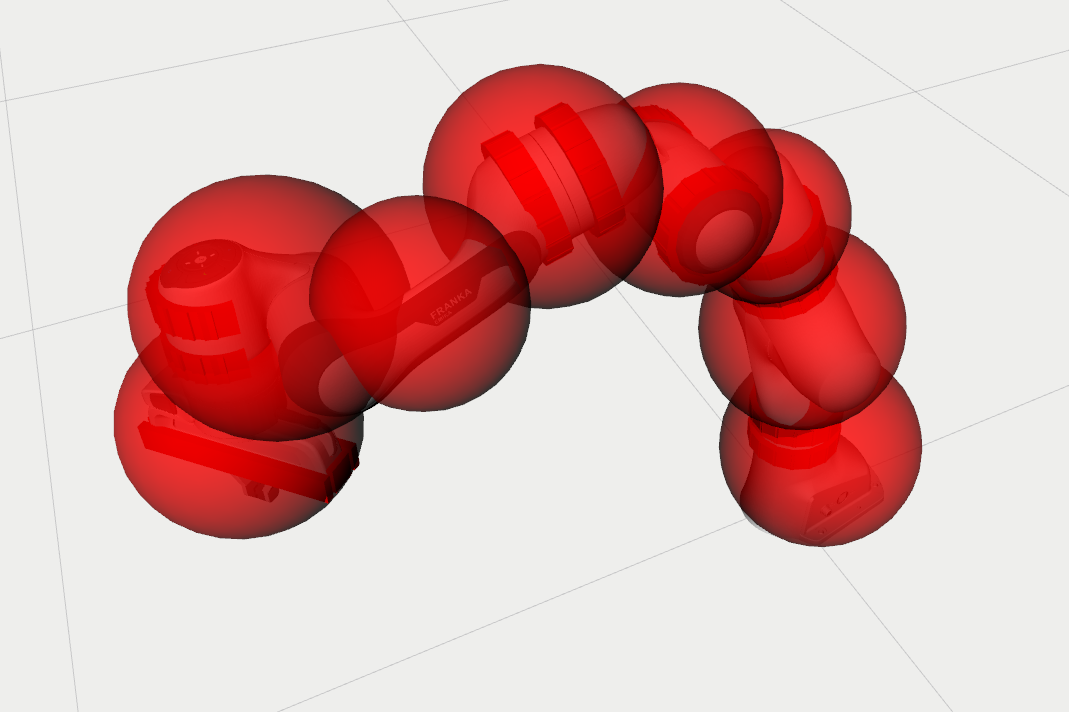
\includegraphics[width=120mm]{figs/spheres.png}
    \end{center}
\label{fig:spheres}
\end{figure}

\begin{lstlisting}[caption={Body and floor points removal and publication \textit{C++} algorithm.},label={lst:pointspublication},captionpos=b]
geometry_msgs::Point point;
ros_robotic_skin::PointArray msg;

ros::Rate rate(50.0);
while (ros::ok())
{
    for (int i = 0; i < num_sensors; i++)
    {
        if (std::isnan(live_points[i].x()) ||
            isInSphere(live_points[i]) || (*\label{code:isInSphere}*)
            (live_points[i].z() < floor_threshold) && removeFloor);
        else
        {
            point.x = live_points[i].x();
            point.y = live_points[i].y();
            point.z = live_points[i].z();
            msg.points.push_back(point);
        }
    }
    pub.publish<ros_robotic_skin::PointArray>(msg);
    msg.points.clear();
    rate.sleep();
}
\end{lstlisting}

Another optional filter that can be applied to the perveived points is that if the boolean variable \lstinline{removeFloor} is set to true, points that are lower than a certain threshold \lstinline{floor_threshold)}, in meters, will also be removed. Also, if a sensor $i$ does not perceive any point in the range for which it is set up, \lstinline{live_point[i]} will be

$$
\begin{bmatrix}
\text{NaN} & \text{NaN} & \text{NaN}
\end{bmatrix}
^{\intercal}
$$

and the point will not be added to the message.

The points are packed in a custom created message called \lstinline{ros_robotic_skin::PointArray} , whose only field is an array of \lstinline{geometry_msgs::Point}s. This is done at \SI{50}{\hertz}, or what is the same, every \SI{20}{\milli \second}.

% TODO
BUFFER IS LEFT

\subsection{Visualization in \textit{rviz}}
\label{ss:visualization}

In this section we extoplain the last step of the perception part: visualization. Visualization of the data perveived by the robot is a very intuitive way of seeing what is going on, both on the perception and control algorithms. We will see how to visualize the data processed by the \lstinline{proximity_listener} node in \textit{rviz}.

There are several dysplay types that can be visualized in rviz. We use \lstinline{Marker Array}s \cite{rvizmarker} to visualize the point cloud generated.

We have called the class that implements the visualization \lstinline{ProximityVisualizer}. In the initializer of the class, shown in listing \ref{lst:proximityinitializer}, the node is suscribed  to the data published in the topic \lstinline{live_points} by \lstinline{proximity_listener}. The data received in that topic will be processed in \lstinline{ProximityVisualizer::Callback}. Next, the publication of messages of type \lstinline{MarkerArray} in the topic \lstinline{visualization_marker_array} is set up. The general properties that are kept through all of the \lstinline{Marker}s that will be added to the \lstinline{MarkerArray} are also set up and the rest of the properties are initialized.

Note that these properties alLow to set up the \lstinline{Marker}'s shape, the size, the color, the coordinates in which it will be located, as well as the frame in which those coordinates are written and the orientation. \lstinline{namespace} allows organization within the same topic so that \lstinline{Marker}s can be further classified. The \lstinline{id} of the marker is unique and whenever a new marker with the same \lstinline{id} is published, the previous one is deleted. Finally, \lstinline{action} can be \lstinline{ADD}, \lstinline{DELETE} or \lstinline{DELETEALL}.

\begin{lstlisting}[caption={Initializer of the ProximityVisualizer class},captionpos=b,label={lst:proximityinitializer}]
ProximityVisualizer::ProximityVisualizer()
{

    sub = n.subscribe<ros_robotic_skin::PointArray>
        ("live_points", 1, &ProximityVisualizer::Callback, this);
    pub = n.advertise<visualization_msgs::MarkerArray>
        ("visualization_marker_array", 1);
    // Marker properties that are the same for all the points
    marker.ns = "Live Points";
    marker.action = visualization_msgs::Marker::ADD;
    marker.scale.x = 0.05;
    marker.scale.y = 0.05;
    marker.scale.z = 0.05;
    marker.color.r = 1.0;
    marker.color.g = 0.0;
    marker.color.b = 0.0;
    marker.color.a = 1.0;
    marker.header.frame_id = "/world";
    marker.type = visualization_msgs::Marker::SPHERE;
    marker.pose.orientation.x = 0.0;
    marker.pose.orientation.y = 0.0;
    marker.pose.orientation.z = 0.0;
    marker.pose.orientation.w = 1.0;
    // Marker properties that depend on the point
    marker.header.stamp = ros::Time::now();
    marker.id = 0;
    marker.pose.position.x = 0.0;
    marker.pose.position.y = 0.0;
    marker.pose.position.z = 0.0;
}
\end{lstlisting}

Every time a new message arrives to the \lstinline{live_points} topic in runtime, the callback will add the new points received  to a \lstinline{MarkerArray}. This is shown in listing \ref{lst:visualizercallback}.

The sequence when a new message arrives is as follows. First, all the previously published markers are deleted publishing a \lstinline{MarkerArray} that contains a \lstinline{Marker} whose \lstinline{action} is \lstinline{DELETEALL}. Then, the new points received are packed into a \lstinline{Marker} and pushed back in a \lstinline{MarkerArray}. Finally, this \lstinline{MarkerArray} is published.

\begin{lstlisting}[caption={Callback of the ProximityVisualizer class},captionpos=b,label={lst:visualizercallback}]
    void ProximityVisualizer::Callback(
        const ros_robotic_skin::PointArray::ConstPtr& msg)
    {
        // Delete all points from previous callback
        marker.action = visualization_msgs::Marker::DELETEALL;
        marker_array.markers.push_back(marker);
        pub.publish<visualization_msgs::MarkerArray>(marker_array);
        marker_array.markers.clear();

        // Add new points
        marker.action = visualization_msgs::Marker::ADD;
        marker.header.stamp = ros::Time::now();
        for (int i = 0; i < msg->points.size(); i++)
        {
            // Check that it's not 'nan' or 'inf'
            marker.id = i;
            marker.pose.position.x = msg->points[i].x;
            marker.pose.position.y = msg->points[i].y;
            marker.pose.position.z = msg->points[i].z;
            marker_array.markers.push_back(marker);
        }
        pub.publish<visualization_msgs::MarkerArray>(marker_array);
        marker_array.markers.clear();
    }
\end{lstlisting}

In order to visualize the \lstinline{MarkerArray}, a subscription to the topic has to be added in \textit{rviz}, as shown in figure \ref{fig:markerarrayrviz}. Since the \lstinline{Namespaces} field is empty, all the points in the received \lstinline{MarkerArray} will be visualized, with no exception.

\begin{figure}[H]
    \caption[Spheres]{
    Menu of the Marker Array plugin in \textit{rviz}.
    }
    \begin{center}
    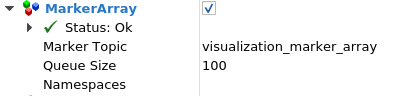
\includegraphics[scale=0.75]{figs/markerarrayrviz.png}
    \end{center}
\label{fig:markerarrayrviz}
\end{figure}

The points are seen in \textit{rviz} as shown in figure \ref{fig:visualizationpoints}, where a wall in front of the robot is being perceived.

\begin{figure}[H]
    \caption[Spheres]{
    Final visualization of the perceived points in \textit{rviz}.
    }
    \begin{center}
    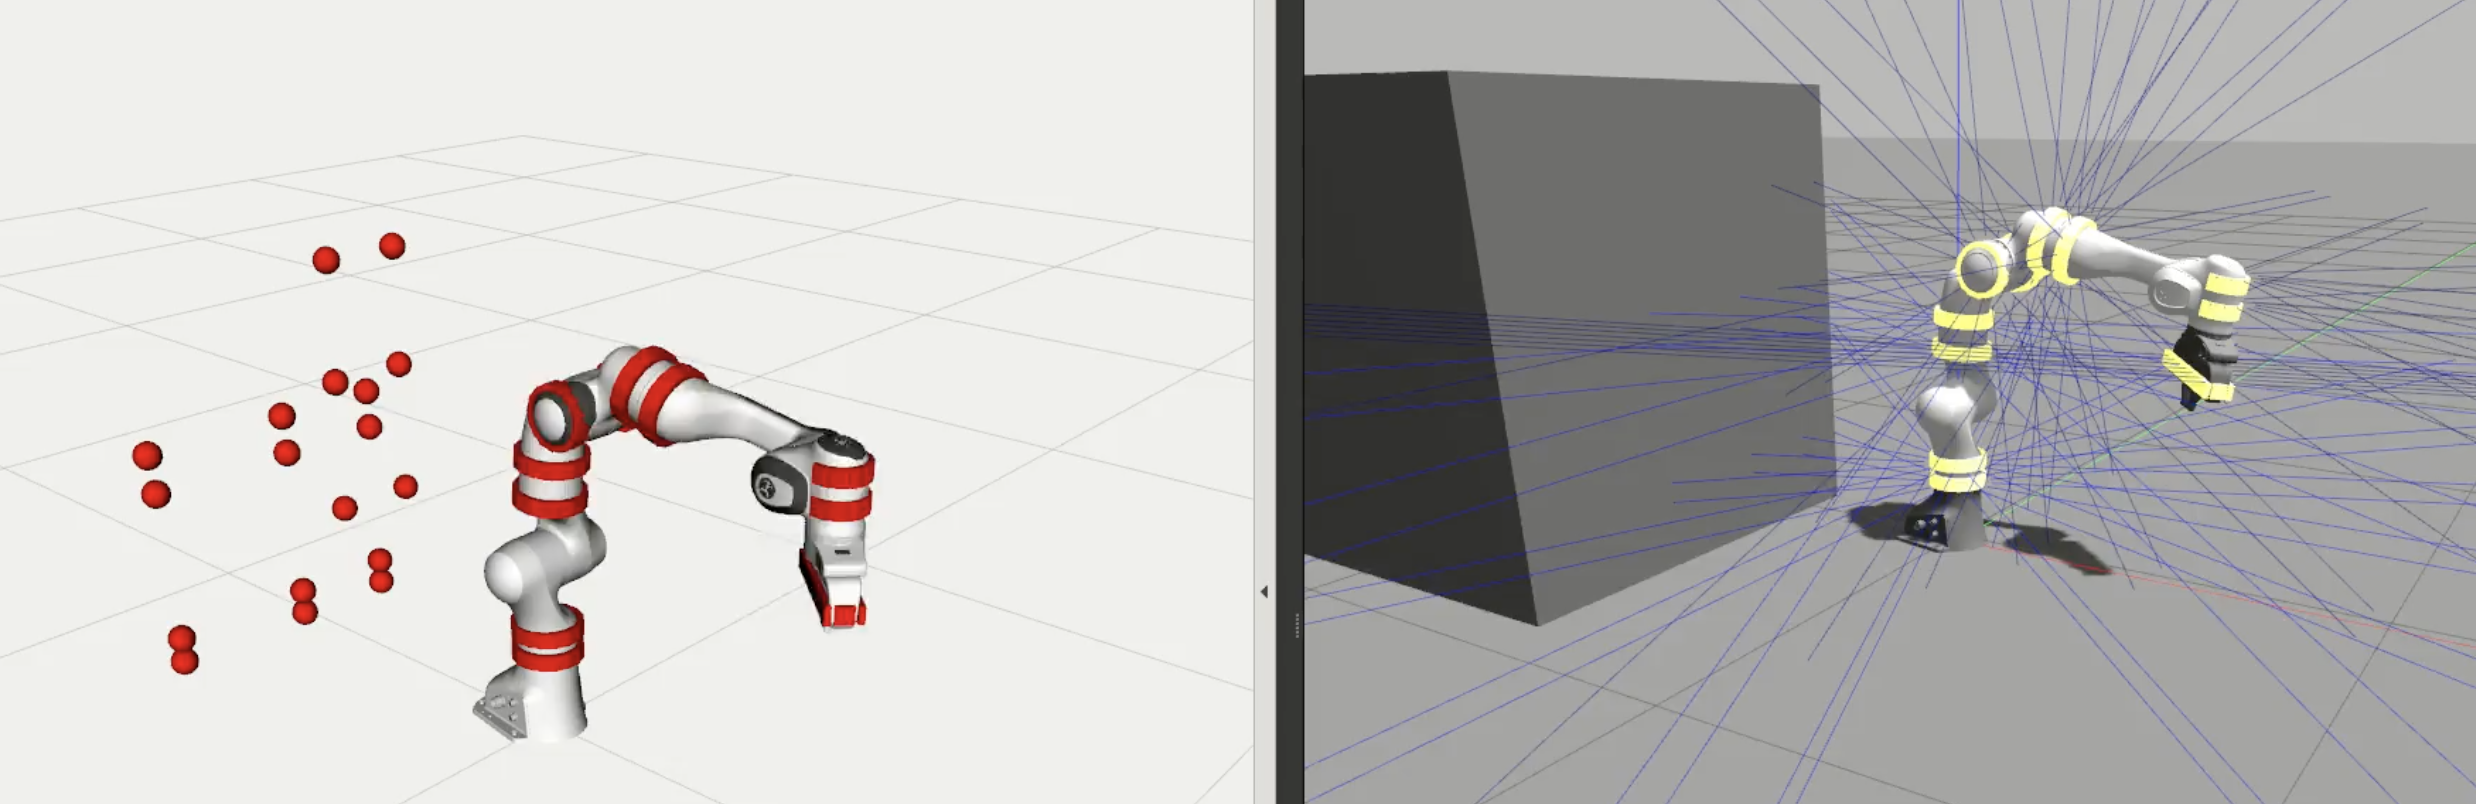
\includegraphics[width=\textwidth]{figs/visualizationpoints.png}
    \end{center}
\label{fig:visualizationpoints}
\end{figure}







\section{Control}
\label{s:control}

% TODO
INTRODUCTORY PARAGRAPH

\subsection{The Kinematic Control Problem}
\label{ss:kinematiccontrol}
In this section one of the most fundamental problems in robotics will be defined and solved: the Kinematic Control Problem. It can be formulated as the problem of obtaining a joint space trajectory $\mathbf{q}(t)$ that satisfies a desired trajectory in the cartesian space $\mathbf{x}(t)$.

This problem contains several elements required in order to solve the collision avoidance problem in subsequent sections. Moreover, the collision avoidance will be built as a modification to the more fundamental method described in this section.

\subsubsection{Geometric representation of the kinematic chain of a robot}
\label{sss:geomrep}

Kinematics is the branch of physics that studies the motion of the bodies. It does that with no consideration of the causes that originate that motion, forces and torques. Kinematics is required and fundamental in robotics for design, analysis, control and simulation.

In order to study the kinematics of a robot its geometric representation must be defined mathematically beforehand. Rigid body kinematics deals with the problem of studying relative movement of two non-deformable elements by attaching a coordinate frame to each of them. Robot manipulators and robots in general can be seen as a series of rigid links connected by joints. Therefore, attaching a frame to each of the links of a robot in a convenient manner is how robots' geometry is usually represented.

However, there are infinitely many ways in which this 3-dimensional frames can be assigned to the links. The origin and rotation of the frames could be located anywhere in the space as long as its movement was fixed to the respective links.

That is where conventions for geometric representation come in place. The most well known and extended convention was introduced by Denavit and Hartenberg (DH) in 1955 \cite{hartenberg1955kinematic}. Although there have been numerous adaptations, the representations serve the same purpose and DH parameters are still widely used. In fact, the manufacturer of the robot employed in this work (\ref{ss:panda}) provides DH parameters in its documentation \cite{FrankaEmikaPanda}.

DH suggest a set of rules to place the frames corresponding to each robot link:

\begin{itemize}
    \item The $n$ links of the mechanism are numbered from 0 to N, being link 0 the fixed base.
    \item The $n$ joints of the mechanism are numbered from 1 to N, with joint $i$ located between links $i-1$ and $i$.
    \item The $\bf{z_i}$ axis is located along the axis of joint $i$.
    \item The $\bf{x_{i-1}}$ axis is located along the common perpendicular between $\bf{z_{i-1}}$ and $\bf{z_i}$ axis.
\end{itemize}

Then, they define 4 parameters that completely define the position and rotation of a link with respect to the previous one. Note that full position and orientation are usually defined by at least 6 parameters. However, geometric constraints inherent to robotic arms allow us to define them with just 4 parameters.

The four parameters are:

\begin{itemize}
    \item $\bf{a_i}$: the distance from $\bf{z_{i-1}}$ to $\bf{z_{i}}$ along $\bf{x_{i-1}}$.
    \item $\bf{\alpha_i}$: the angle from $\bf{z_{i-1}}$ to $\bf{z_{i}}$ about $\bf{x_{i-1}}$.
    \item $\bf{d_i}$: the distance from $\bf{x_{i-1}}$ to $\bf{x_{i}}$ along $\bf{z_{i}}$.
    \item $\bf{\theta_i}$: the angle from $\bf{x_{i-1}}$ to $\bf{x_{i}}$ about $\bf{z_{i}}$.
\end{itemize}

Most common joint types in robot manipulators are revolute and prismatic joints. In the case of \textbf{revolute joints} all the parameters but $\bf{\theta_i}$ are defined by the geometric design of the robot, while $\bf{\theta_i}$ is the variable of the movement. If the joint is \textbf{prismatic}, all the parameters but $\bf{d_i}$ are defined by the geometry of the robot, while $\bf{d_i}$ is the variable of the movement.

Franka Panda Emika (described in section \ref{ss:panda}) is equipped with 7 revolute joints. Its DH parameters are given by the manufacturer and shown in figure \ref{fig:FEPchain}.

In ROS, the robots' geometry is internally described in \textit{urdf} files. \textit{urdf} files make use of \textit{Extensible Markup Language (XML)}, the same markup language that is used for web pages in \textit{html} files. The following fragment taken from the complete descripion of Franka Panda (by justagist \cite{justagist}) Emika describes the transformation from frame $6$ to frame $7$.

\begin{lstlisting}[caption={Fragment of panda\_arm.urdf},captionpos=b]
<joint name="${arm_id}_joint7" type="revolute">
      <safety_controller k_position="100.0"
                         k_velocity="40.0"
                         soft_lower_limit="-2.8973"
                         soft_upper_limit="2.8973"/>
      <origin rpy="${pi/2} 0 0" xyz="0.088 0 0"/> (*\label{code:origin}*)
      <parent link="${arm_id}_link6"/>
      <child link="${arm_id}_link7"/>
      <axis xyz="0 0 1"/>
      <limit effort="12" lower="-2.8973"
                         upper="2.8973"
                         velocity="2.6100"/>
      <dynamics damping="1.0" friction="0.5"/>
</joint>
\end{lstlisting}

The relative positions and orientations are defined under the tag \lstinline{<origin/>} in line \ref{code:origin}. DH parameters are not used in this tag, even though \textit{urdf} could be adapted to use them through the language \textit{xacro}, that permits to do math inside textit{urdf}. Rotation is defined through \textit{Euler Angles}:  rotations are defined by applying rotation about $x$, $y$ and $z$ axes, in this order. Translation is defined with a $3 \times 1$ vector that goes from frame $i-1$ to frame $i$, from $6$ to $7$ in this case.

The use of DH parameters would have been beneficial and less error prone through the process of writing the \textit{urdf} description.

In the next section we will make use of the geometric representation of the robot to locate the diferent elements of the robot.

\subsubsection{Forward Kinematics}
\label{sss:FK}

Forward kinematics provides a mathematical tool that allows to find the position and orientation of the end effector or any other point in the kinematic chain given all the joint variables' values. These are ($\bf{\theta_i}$s for revolute joints and $\bf{d_i}$s for prismatic joints.

A common way to represent the rotation and translation from one axis to another are homogeneous transformation matrices. They are $4 \times 4$ matrices defined as in equation \ref{e:transformationmatrix}.

\begin{equation}
    \label{e:transformationmatrix}
    ^{i-1}\mathbf{T}_{i} = \left(\begin{array}{cc}
    ^{i-1} \mathbf{R}_{i} & ^{i-1} \boldsymbol{p}_{i} \\
    \mathbf{0}^{\mathrm{T}} & 1
    \end{array}\right)
\end{equation}

The top left $3 \times 3$ matrix $^{i-1} \mathbf{R}_{i}$ defines the rotation from axis $i-1$ to axis $i$. $^{i-1} \mathbf{R}_{i}$ is an orthogonal matrix, this meaning that the basis formed by its columns is orthonormal. Each of the column vectors are required to have unit length. One nice property of orthogonal matrices is that their inverse is exactly the same as their transpose:

$$(^{i-1} \mathbf{R}_{i})^{-1} = ^{i} \mathbf{R}_{i-1} = (^{i-1} \mathbf{R}_{i})^{\intercal}$$

On the other hand, the top right $3 \times 1$ position vector $^{i-1} \boldsymbol{p}_{i}$ defines the translation vector from axis $i-1$ to axis $i$.

Homogeneous transformation matrices are an easy and convenient way to calculate several linked transformations. $^{i-2}\mathbf{T}_{i}$ would be calculated as follows:

$$^{i-2}\mathbf{T}_{i} = ^{i-2}\mathbf{T}_{i-1} ^{i-1}\mathbf{T}_{i} =
    \left(\begin{array}{cc}
    ^{i-2} \mathbf{R}_{i-1} & ^{i-2} \boldsymbol{p}_{i-1} \\
    \mathbf{0}^{\mathrm{T}} & 1
    \end{array}\right)
    \left(\begin{array}{cc}
    ^{i-1} \mathbf{R}_{i} & ^{i-1} \boldsymbol{p}_{i} \\
    \mathbf{0}^{\mathrm{T}} & 1
    \end{array}\right) =
    \left(\begin{array}{cc}
    ^{i-2} \mathbf{R}_{i-1} ^{i-1} \mathbf{R}_{i} & (^{i-2} \boldsymbol{p}_{i-1} +  ^{i-2} \mathbf{R}_{i-1} ^{i-1} \boldsymbol{p}_{i})\\
    \mathbf{0}^{\mathrm{T}} & 1
    \end{array}\right)
$$

This is the desired behaviour because $^{i-2} \mathbf{R}_{i-1} ^{i-1} \mathbf{R}_{i}$ represents the combination of applying the rotation $^{i-2} \mathbf{R}_{i-1}$ first and $^{i-1} \mathbf{R}_{i}$ after. $(^{i-2} \boldsymbol{p}_{i-1} +  ^{i-2} \mathbf{R}_{i-1} ^{i-1} \boldsymbol{p}_{i})$ takes the vector $^{i-1} \boldsymbol{p}_{i}$ to the $i-2$ basis and them it sums the origin of the frame $i-1$, $^{i-2} \boldsymbol{p}_{i-1}$, already written in the $i-2$ axis.

The homogeneous transformation matrix $^{i-1}\mathbf{T}_{i}$ can be built from the DH parameters representation with $\bf{a_i}$, $\bf{\alpha_i}$, $\bf{d_i}$ and $\bf{\theta_i}$. For that purpose the following steps are combined in order:
\begin{enumerate}
    \item $\bf{\alpha_i}$ rotation about the axis $x_{i-1}$.
    \item $\bf{a_i}$ translation through the axis $x_{i-1}$.
    \item $\bf{\theta_i}$ rotation about the axis $z_{i}$.
    \item $\bf{d_i}$ translation about the axis $z_{i}$.
\end{enumerate}


$$
^{i-1}\mathbf{T}_{i} =
\left(\begin{array}{cccc}
1 & 0 & 0 & 0 \\
0 & \cos \alpha_{i} & - \sin \alpha_{i} & 0 \\
0 & \sin \alpha_{i} & \cos \alpha_{i} & 0 \\
0 & 0 & 0 & 1
\end{array}\right) \cdot
\left(\begin{array}{cccc}
1 & 0 & 0 & a_{i} \\
0 & 1 & 0 & 0 \\
0 & 0 & 1 & 0 \\
0 & 0 & 0 & 1
\end{array}\right) \cdot
\left(\begin{array}{cccc}
\cos \theta_{i} & - \sin \theta_{i} & 0 & 0 \\
\sin \theta_{i} & \cos \theta_{i} & 0 & 0 \\
0 & 0 & 1 & 0 \\
0 & 0 & 0 & 1
\end{array}\right) \cdot
\left(\begin{array}{cccc}
1 & 0 & 0 & 0 \\
0 & 1 & 0 & 0 \\
0 & 0 & 1 & d_{i} \\
0 & 0 & 0 & 1
\end{array}\right)
$$

$$
=
\left(\begin{array}{cccc}
\cos \theta_{i} & -\sin \theta_{i} & 0 & a_{i} \\
\sin \theta_{i} \cos \alpha_{i} & \cos \theta_{i} \cos \alpha_{i} & -\sin \alpha_{i} & -\sin \alpha_{i} d_{i} \\
\sin \theta_{i} \sin \alpha_{i} & \cos \theta_{i} \sin \alpha_{i} & \cos \alpha_{i} & \cos \alpha_{i} d_{i} \\
0 & 0 & 0 & 1
\end{array}\right)
$$

Once all the the transformation matrices $^{i-1}\mathbf{T}_{i}$ are defined for $i = 1,  \dots, n$, the full transformation from the base $i=0$ to the end effector $i=n$ transformation can easily be calculated:

$$
^{0}\mathbf{T}_{n} = ^{0}\mathbf{T}_{1} ^{1}\mathbf{T}_{2} \dots ^{n-1}\mathbf{T}_{n}
$$

Forward Kinematics are calculated in the robot\_state\_publisher package \cite{rosstatepublisher}. The robot's description is read from a \textit{urdf} file loaded in the parameter server. Then, the joints' values are read from a topic named \textit{/joint\_states} and used to compute forward kinematics of all the joints. The results are published in a topic named \textit{/tf}.

\subsubsection{Inverse Kinematics}
\label{sss:IK}

The inverse Kinematics problem is the opposite to the one of Forward Kinematics (section \ref{sss:FK}). The objective in this case is not to locate the robot's parts once known joint values, but to find the joint values take the end effector (or any other point in the kinematic chain) to a given position and orientation.

Given the nature of the homogeneous transformation matrices defined in section \ref{sss:FK}, whose elements contain $\sin$ and $\cos$ functions, the problem requires to solve a set of non linear equations defined by:

$$
^{0}\mathbf{T}_{n}(q_{1}, \dots, q_{n}) = (^{0}\mathbf{T}_{n})^{d}
$$

It is trivial to see that solving the position $^{0} \boldsymbol{p}_{n}(q_{1}, \dots, q_{n}) = (^{0} \boldsymbol{p}_{n})^{d}$ describes $3$ equations. On the other hand, since rotation matrices provide six auxiliary relationships ($3$ coming from the fact that column vectors to have unit length, and $3$ coming from the requirement of its column vectors being mutually orthogonal), and they contain $9$ elements, $9 - 6 = 3$ more equations are coming from $^{0} \mathbf{R}_{n}(q_{1}, \dots, q_{n}) = (^{0} \mathbf{R}_{n})^{d}$.

In order a solution to exist, the desired location and rotation $(^{0}\mathbf{T}_{n})^{d}$ needs to be in the robot's workspace.

A closed form of the equation does not always exist. In fact, in the common case there is no way to do this. Consequently, numerical methods are needed.

For Franka Panda Emika $n = 7$, there are infinitely many joint values that satisfy the Inverse Kinematics equations.

\subsubsection{Forward Instantaneous Kinematics}

\label{sss:FIK}

Forward instataneous Kinematics relates the motion rates of joints $\mathbf{q} = \begin{bmatrix}q_{1} & \dots & q_{n}\end{bmatrix}^{\intercal}$ with the velocities in the 3D Cartesian Space of the end effector.

Note that everything defined for the specific point in the kinematic chain \textit{end effector} will also be adaptable to any other point in the kinematic chain, by simply considering a reduced kinematic chain that goes from the base to joint $i$, instead of to the end effector.

We start by redefining what we got in section \ref{sss:FK}. This was our final result, given in the form of homogeneous transformation matrices:

$$
^{0}\mathbf{T}_{n} = ^{0}\mathbf{T}_{1} ^{1}\mathbf{T}_{2} \dots ^{n-1}\mathbf{T}_{n} =
\left(\begin{array}{cc}
    ^{0} \mathbf{R}_{n} & ^{0} \boldsymbol{p}_{n} \\
    \mathbf{0}^{\mathrm{T}} & 1
\end{array}\right)
$$

The position of the end effector is well defined by the position vector $^{0} \boldsymbol{p}_{n}$. However, the rotation matrix $^{0} \boldsymbol{p}_{n}$, by definition of rotation matrix, contains six auxiliary relationships (\ref{sss:FK}). In consequence, rotation matrices are not minimal representations. For Forward Instantaneous Kinematics we will use a minimal representation of orientation, such as Euler angles (\ref{sss:geomrep}), where orientation is completely described with just three elements.

$$\mathbf{t}(t) = \mathbf{f}(t) = \begin{bmatrix} f_{1}(t) \\ f_{2}(t) \\ f_{3}(t) \\ f_{4}(t) \\ f_{5}(t) \\ f_{6}(t) \end{bmatrix}
$$

$\mathbf{f}$ is a differentiable nonlinear vector function. $f_{1}(t)$, $f_{2}(t)$ and $f_{3}(t)$ describe the position of the end effector and $f_{4}(t)$ $f_{5}(t)$ and $f_{6}(t)$ its orientation.

Thus, the rate of change of this parameters is given by $\mathbf{\dot{t}}(t)$,

$$
\label{asdf}
{\dot{t}_i}(t) = \frac{d{{t}_i}(t)}{dt} = \sum_{i=1}^{n} \frac{\partial{{t}_i}}{\partial q_i} \cdot \frac{dq_i}{dt} = (\nabla_{\mathbf{q}}{t}_i)^{\intercal} \cdot \mathbf{\dot{q}}
$$

In matrix form,

$$
\mathbf{\dot{t}} = \frac{d\mathbf{{t}}}{dt} =
[
    \frac{\partial{\mathbf{t}}}{\partial \mathbf{q}}
]
\cdot \mathbf{\dot{q}} =
\mathbf{J}_{\mathbf{t}}(\mathbf{{q}}) \cdot \mathbf{\dot{q}}
$$

$\mathbf{J}_{\mathbf{t}}(\mathbf{{q}}) \in \mathbb{R}^{6 \times n}$ is called the \textit{Jacobian}. It relates joint space velocities to cartesian space velocities and it is a function of the joint angles (or distances in the case of prismatic joints) $\mathbf{{q}}$. Its $i$th row is the gradient of the component $i$ in $\mathbf{t}(t)$ $\nabla_{\mathbf{q}}{t}_i$.

It is convenient to remark that, with this formulation, the components of the velocity vector $\mathbf{\dot{t}}(t)$ express the rate of change of the parameters that form the minimal representation vector $\mathbf{t}(t)$. In Rigid Body Kinematics, the velocities of all the points in a rigid body (a link in our case) are completely defined by two vectors \cite{Ruigomez2010}.

\begin{enumerate}
    \item The \textit{angular velocity} of the body $\mbox{\boldmath$\omega$}$.
    \item The velocity of one point pertaining to the body $\mathbf{v}_{O}$.
\end{enumerate}

Given those two vectors the velocity $\mathbf{v}_{P}$ of any other point $P$ pertaining to the same body can be calculated as:

\begin{equation}
\label{eq:velfield}
\mathbf{v}_{P} = \mathbf{v}_{O} + \mbox{\boldmath$\omega$} \times \overrightarrow{\mathbf{OP}}
\end{equation}

However, while the end effector velocity represented by the first three elements of $\mathbf{\dot{t}}(t)$ is suitable for $\mathbf{v}_{O}$, the last three elements of $\mathbf{\dot{t}}(t)$ don't express the angular velocity $\mbox{\boldmath$\omega$}$ of the end effector link. They represent the rate of change of Euler Angles or any other minimal representation parameters chosen to describe orientation.

The actual Jacobian that relates the joint space velocities to $\mathbf{\dot{x}} = \begin{bmatrix} \mathbf{v}_{\text{end effector}} \\ \mbox{\boldmath$\omega$}_{\text{end effector}} \end{bmatrix}$ is:

$$
\mathbf{J}(\mathbf{{q}}) = \mathbf{T}(t) \cdot \mathbf{J}_{\mathbf{t}}(\mathbf{{q}})
$$

$$
\mathbf{T}(t) = \begin{bmatrix}\mathbf{I} & \mathbf{0} \\ \mathbf{0} & \mathbf{R}(t)\end{bmatrix}
$$

$\mathbf{T}(t)$ only depends on time $t$ and its expression depends on the minimal representation chosen to describe orientation. The resulting equation is:

\begin{equation}
    \label{eq:FIK}
    \mathbf{\dot{x}} = \mathbf{J}(\mathbf{{q}}) \cdot \mathbf{\dot{q}}
\end{equation}

There are many methods that compute the values of the jacobian matrix $\mathbf{J}(\mathbf{{q}})$ \cite{Orin1984}. The general idea underlying is similar in all of them, with differences in efficiency.

$$
\mathbf{J}(\mathbf{{q}}) = \begin{bmatrix} \mbox{\boldmath$\mathcal{J}$}_{P1} & \mbox{\boldmath$\mathcal{J}$}_{P2} & \dots & \mbox{\boldmath$\mathcal{J}$}_{Pn} \\  \mbox{\boldmath$\mathcal{J}$}_{O1} & \mbox{\boldmath$\mathcal{J}$}_{O2} & \dots & \mbox{\boldmath$\mathcal{J}$}_{On} \end{bmatrix}
$$

$\mbox{\boldmath$\mathcal{J}$}_{Pi} \in \mathbb{R}^{3 \times 1}$ denotes the contribution of $\dot{q}_i$ per radian to $\mathbf{v}_{\text{end effector}}$. $\mbox{\boldmath$\mathcal{J}$}_{Oi} \in \mathbb{R}^{3 \times 1}$ denotes the contribution of $\dot{q}_i$ per radian to $\mbox{\boldmath$\omega$}_{\text{end effector}}$. Their value is computed as follows:

$$
\boldsymbol{J}_{P i}=\left\{\begin{array}{ll}
^{0}\mathbf{z}_{i-1} & \text { if joint } i \text { is prismatic } \\
^{0}\mathbf{z}_{i-1} \times ^{i-1}\boldsymbol{p}_{\text{end effector}} & \text { if joint } i \text { is revolute }
\end{array}\right.
$$

$$
\boldsymbol{J}_{O i}=\left\{\begin{array}{ll}
\mathbf{0} & \text { if joint } i \text { is prismatic } \\
^{0}\mathbf{z}_{i-1} & \text { if joint } i \text { is revolute }
\end{array}\right.
$$

As described in section \ref{sss:geomrep}, $^{0}\mathbf{z}_{i-1}$ is joint $i$'s $z$ axis, which is a unitary vector in the direction of the joint. $^{0}\mathbf{z}_{i-1}$ coincides both the direction in which a prismatic joint contributes to the end effector velocity $\mathbf{v}_{\text{end effector}}$ and with the contribution of a revolute joint to the angular velocity of the end effector $\mbox{\boldmath$\omega$}_{\text{end effector}}$. The magnitude $\mathbf{z}_{i-1} \times ^{i-1}\boldsymbol{p}_{\text{end effector}}$ is due to the $\mbox{\boldmath$\omega$} \times \overrightarrow{\mathbf{OP}}$ part in equation \ref{eq:velfield}. It is obvious that the contribution of a prismatic joint to $\mbox{\boldmath$\omega$}_{\text{end effector}}$ is $\mathbf{0}$.

KDL

\subsubsection{Inverse Instantaneous Kinematics}
\label{sss:IIK}
As defined at the beginning of \ref{ss:kinematiccontrol}, the kinematic control problem deals with the problem of obtaining a joint space trajectory $\mathbf{q}(t)$ that satisfies a desired trajectory in the cartesian space $\mathbf{x}(t)$. Several approaches can be taken in order to find a solution to this problem, but according to \cite{siciliano1990kinematic}, the most relevant ones for redundant manipulators (sections \ref{ss:panda} and \ref{sss:FK}) solve the problem at the joint velocity level.

Therefore, joint space velocities $\mathbf{\dot{q}}(t)$ that result in end effector velocities $\mathbf{\dot{x}_{d}}$ that satisfy a desired trajectory in the cartesian space $\mathbf{x_{d}}(t)$ must be found. This is the opposite problem to the one presented in the previous section (\ref{sss:FIK}) that was resolved in equation \ref{eq:FIK}. The equation presents a linear system of equations in the unknowns ${\mathbf{\dot{q}}}$. This contrasts with the fact that, as stated in section \ref{sss:IK}, the Inverse Kinematics problem is non-linear. The jacobian ${\mathbf{J}(\mathbf{{q}})}$ is a local linearization of the instantaneous problem, which is valid only for the specific time instant $t$ and joint values $\mathbf{{q}}$ for which it was calculated. In the general task that than be identified by $m$ variables:

\begin{equation}
    \label{eq:linearEquations}
    \underset{m\times n}{\mathbf{J}(\mathbf{{q}})} \cdot  \underset{n\times 1}{\mathbf{\dot{q}}} = \underset{m\times 1}{\mathbf{\dot{x}_{d}}}
\end{equation}

It is important to note that the maximum number of variables a task can be identified with is $m = 6$. This implies that for a redundant robot for which $n >= 7$, $m > n$ will always remain true.

In the following paragraphs we will utilize some definitions and theorems of Linear Algebra to verify that the linear system of equations defined by equation \ref{eq:linearEquations} has a set of solutions that can only be either empty or infinite. We also verify that when the ${\mathbf{J}(\mathbf{{q}})}$ is full rank, i.e. when its rank is exactly $m$, the vector space of solutions has dimension $(m-n)$. When the rank is $<m$, there exists no solution.

We start by listing some definitions and theorems of Linear Algebra (taken from \cite{hefferonlinear}. However this are well known results and definitions and can be found in any general linear algebra book).

% \begin{definition}
% A \textbf{linear combination} of \( x_{1}, \ldots, x_{n} \) has the form
% $
% a_{1} x_{1}+a_{2} x_{2}+a_{3} x_{3}+\dots+a_{n} x_{n}
% $,
% where the numbers \( a_{1}, \ldots, a_{n} \in \mathbb{R} \) are the combination's coefficients.
% \end{definition}

% \begin{definition}
% The \textbf{span} of a nonempty subset \( \mathcal{S} \) of a vector space is the set of all linear combinations of vectors from \( \mathcal{S} \).
% \[
% [\mathrm{S}]=\left\{\mathrm{c}_{1} \vec{s}_{1}+\cdots+\mathrm{c}_{n} \vec{s}_{n} \mid \mathrm{c}_{1}, \ldots, \mathrm{c}_{n} \in \mathbb{R} \text { and } \vec{s}_{1}, \ldots, \vec{s}_{n} \in \mathrm{S}\right\}
% \]
% \end{definition}

\begin{definition}
The \textbf{row space}/\textbf{column space} of a matrix is the span of the set of its rows/columns. The \textbf{row rank}/\textbf{column rank} is the dimension of this space, the number of linearly independent rows/columns.
\end{definition}

\begin{theorem}
For any matrix, the row rank and column rank are equal.
\end{theorem}

\begin{definition}
The \textbf{rank} of a matrix is its row rank or its column rank.
\end{definition}

\begin{theorem}
No linearly independent set can have a size greater than the dimension of the enclosing space.
\end{theorem}

Therefore, because of this last theorem, it is obvious that the maximum rank for a given matrix $\mathbf{A} \in \mathbb{R}^{m \times n} $ is the minimum value between $m$ and $n$. The rank of this matrix can only be equal to or less than that maximum rank. In the case of redundant robots, the maximum rank ${\mathbf{J}(\mathbf{{q}})}$ will always be given by the dimension of the row space $m$, that is, the number of variables needed to define the task.

\begin{theorem}
For linear systems with $n$ unknowns and with matrix of coefficients $\mathbf{A}$, the statements
\begin{enumerate}
    \item the rank of $\mathbf{A}$ is $r$
    \item the vector space of solutions of the associated homogeneous system has dimension $(n$-$r)$
\end{enumerate}
are equivalent.
\end{theorem}

Consequently, the homogeneous system associated to equation \ref{eq:linearEquations}, ${\mathbf{J}(\mathbf{{q}})} \cdot  {\mathbf{\dot{q}}} = {\mathbf{0}}$, has a solution space of dimension $(\text{n} - \text{r}) \geq (\text{n} - \text{max}({\text{r}})) = (\text{n} - \text{m})$. In the case of Panda Franka Emika, the solution space of the associated homogeneous system will always be greater than or equal to $1$: $(\text{n} - \text{r}) \geq (\text{n} - \text{max}(\text{m})) = (7-6)$.

However, the existance of solution to the general equation requires a particular solution to exist also, because of the following theorem:

% Please add the following required packages to your document preamble:
% \usepackage{multirow}
\begin{table}[]
    \caption{Number of solutions of a linear system}
    \centering
    \label{tab:numbersolutions}
    \begin{tabular}{ll|l|l|}
    \cline{3-4}
                                                                                                                                & \multicolumn{1}{c|}{} & \multicolumn{2}{c|}{\textbf{\begin{tabular}[c]{@{}c@{}}number of solution of \\ the homogeneous system?\end{tabular}}} \\ \cline{3-4}
    \multicolumn{1}{c}{}                                                                                                        &                       & \textbf{one}                                           & \textbf{infinitely many}                                         \\ \hline
    \multicolumn{1}{|l|}{\multirow{2}{*}{\textbf{\begin{tabular}[c]{@{}l@{}}a particular \\ solution exists?\end{tabular}}}} & \textbf{yes}          & unique solution                                        & infinitely many solutions                                        \\ \cline{2-4}
    \multicolumn{1}{|l|}{}                                                                                                      & \textbf{no}           & no solutions                                           & no solutions                                                     \\ \hline
    \end{tabular}
\end{table}

% TODO
\textbf{PROVE THAT IF} $r < m$ no particular solution exists.
For a linear system of equations Ax = b, a solution exists for all b if and only if the rank of A is equal to the dimension of b, i.e, A is full rank.

Therefore when the rank of ${\mathbf{J}(\mathbf{{q}})}$ becomes smaller than $m$, the ability to control one axis either of translation or rotation is lost. The positions $q$ in which this situation is given are called singularities.

Summing up, the problem has been defined as a set of linear equations (equation \ref{eq:linearEquations}) and the existance of the solutions has been studied until now. Next, we must find a solution to the set of equations.

% TODO

Pseudoinverse

However, doesn't avoid singularities.

% TODO
\textbf{NUMERIC INSTABILITY SINGULARITIES OF PSEUDOINVERSE}. Probably dividing something by zero.

The reader may think that it would be useful to have a measure of when one of this situations is about to take place. \cite{yoshikawa1985dynamic} introduced a measure that indicates how close a robot is from a singularity:

$$\sqrt{\mathbf{J^{\intercal}} \cdot \mathbf{J}}$$

This value tends to $0$ when the vector $q$ tends to a position in which the rank of $\mathbf{J}$ will be decreased.

\textbf{GENERAL SOLUTION OF THE EQUATION}

% TODO
\textbf{Leageouis and middle range of the joints}


\subsubsection{End effector Position Control through Inverse Instantaneous Kinematics}
\label{sss:eepositioncontrol}


\begin{lstlisting}[caption={CartesianPositionController.cpp},captionpos=b]
void moveToPosition(const Eigen::Vector3d xd)
{
    Eigen::VectorXd qDot;
    positionErrorVector = xd - x;

    while (positionErrorVector.norm() > position_error_threshold
            && ros::ok())
    {
        readEndEffectorPosition();
        readControlPointPositions();
        positionErrorVector = xd - x;
        xdDot = pGain * positionErrorVector;
        ros::spinOnce();
        qDot = IIK(xdDot)
        jointVelocityController.sendVelocities(qDot);
        rate.sleep();
    }
    qDot = Eigen::VectorXd::Constant(7, 0.0);
    jointVelocityController.sendVelocities(qDot);
}

Eigen::VectorXd IIK(Eigen::Vector3d xdDot)
{
    J = kdlSolver.computeJacobian("end_effector", q);
    Jpinv = J.completeOrthogonalDecomposition().pseudoInverse();
    Eigen::VectorXd qDot1, qDot2;
    qDot1 = Jpinv * xdDot;
    qDot2 = secondaryTaskGain *
            ((Eigen::MatrixXd::Identity(7,7) - Jpinv*J) *
            secondaryTaskFunctionGradient(q));
    return qDot1 + qDot2;
}

Eigen::VectorXd secondaryTaskFunctionGradient(Eigen::VectorXd q)
{
    Eigen::VectorXd qMid, qRanges;
    qMid = 0.5 * (jointLimitsMax + jointLimitsMin);
    qRanges = jointLimitsMax - jointLimitsMin;
    return 2.0/7.0 * (q - qMid).cwiseQuotient(qRanges);
}
\end{lstlisting}

\subsection{Collision avoidance algorithm based on potential field methods and joint velocity constraints}
\label{ss:flacco}

The method presented in this section is an adaptation of the academic article ``A Depth Space Approach to Human-Robot Collision Avoidance'' \cite{flacco2012depth}, published by F. Flacco et al. in 2012. The paper presents an avoidance algorithm that takes depth images as inputs. In this work we have implemented the same functionality leveraging the perception via proximity sensing presented in section \ref{s:perception} instead.

The objective of the control algorithm is to maintain a main task as long as collision can be avoided. For that purpose, a disctintion is made between a discrete set of points in the robot kinematic chain that are taken to avoid the collision of any part of the robot with an object in its surroundings. On the one hand, there is the end effector point. This point is given a special attention due to the fact that the main task of a robot is usually focused on employing its end effector to accomplish a specific goal controlling its motion. On the other hand, there are a set of points along the robot, which are selected to represent the whole body of the robot and are treated differently.

The end effector algorithm is based on a \textbf{potential field} approach, where two kinds of virtual fields are generated to accomplish the goal of completing a main task while avoiding collision. Attractive fields contribute to movement towards the goal, while repulsive fields avoid getting closer to a possible collision. This algorithm is further explained in section  \ref{sss:flaccorepulsive}.

The other control points are treated as cartesian constraints that are translated into \textbf{joint velocity constraints} that are satisfied using the task redundancy of the robot. The authors state that if the had considered the same approach for them, they would have had to prioritize the tasks of some points over the rest so that the problem turned feasible. However, doing this is problematic in their own words: giving priority to the end effector the collision safety of the points in the body would not be guaranteed, whereas not prioritizing it would result in random end effector trajectories that would not accomplish the task. This is addressed in section \ref{sss:flaccobody}.

\subsubsection{Potential field methods and velocity estimation applied to the effector}
\label{sss:flaccorepulsive}

\blindtext

\subsubsection{Joint velocity constraints to avoid collision of any point in the robot}
\label{sss:flaccobody}

\blindtext

\subsection{Optimization based collision avoidance algorithm}
\label{ss:optimization}

% TODO: Introductory paragraph

\blindtext

\subsubsection{Introduction to Mathematical Optimization and Quadratic Programming}
\label{sss:optimizationintro}

\textbf{Mathematical Optimization}, also called \textbf{Mathematical Programming}, is the set of principal methods used to determine the best solutions to mathematically described problems.

Formally speaking, Mathematical Optimization is the process of the formulation and solution of a optimization problem of the general mathematical form:

$$
\underset{\text { w.r.t. } \mathbf{x}}{\text{minimize}} \, f(\mathbf{x}), \mathbf{x}=\left[x_{1}, x_{2}, \ldots, x_{n}\right]^{T} \in \mathbb{R}^{n}
$$

subject  to  the  constraints:

% Column vector
$$
\begin{array}{ll}
    g_{j}(\mathbf{x}) \leq 0, & j=1,2, \ldots, m \\
    h_{j}(\mathbf{x})=0, & j=1,2, \ldots, r
\end{array}
$$

$f(\mathbf{x})$, $g_{j}(\mathbf{x})$ and $h_{j}(\mathbf{x})$ are scalar functions of a vectorial variable $\mathbf{x}$. The components $x_i$ of $\mathbf{x}$ are called the \textit{variables of the optimization problem}, $f(\mathbf{x})$ is the \textit{objective function}, $g_{j}(\mathbf{x})$ are the \textit{inequality constraint functions} and $h_{j}(\mathbf{x})$ are the \textit{equality constraint functions}. The optimum vector $\mathbf{x}$ that solves the optimization problem is denoted with an asterisk $\mathbf{x^{*}}$ and the corresponding \textit{optimal objective function value }is $f(\mathbf{x^{*}})$.

Optimization problems are usually solved using \textit{optimization algorithms}. These optimization algorithms are tailored to particular types of optimization problems. This is why classification of optimization models is a crucial part in the optimization problem.

One important optimization problem type is the Quadratic Programming (QP) problem. It is an important class of problem on its own and also a subproblem for more general constrained optimization problems (sequential quadratic programming (SQP), augmented Lagrangian methods). These are the characteristics of QP problems:

\begin{itemize}
    \item \textbf{One objective function}. The most common case is the problem being defined by a single objective function, but there are also problems that can be modeled with no objective functions or using many of them.
    \item \textbf{Deterministic optimization}. Depending on the nature of the data, an optimization problem can be either \textit{deterministic} or \textit{stochastic}. Due to measurement errors or more importantly because the data being used is data that represents the future, uncertainty has to be incorpored to the model. In that case we are talking about stochastic optimization. On the other hand, if data is assumed to be known with accuracy we are talking about deterministic optimization.
    \item \textbf{Continuous optimization problem}. For some problems, the variables of the optimization problem can only take values from a discrete set, often a subset of integers, whereas for other problems they can take any value in $\mathbb{R}$. The former are called \textit{discrete optimization problems} and the latter are called \textit{continuous optimization problems}. Continuous optimization problems tend to be easier to solve because the continuity of the functions involved can be used to obtain information about the neighbourhood of the current value.
    \item \textbf{Constrained optimization}. Sometimes there problem does not require to specify constraints for the variables of the optimization problem. When this is the case we are talking about \textit{unconstrained optimization}. If the problem requires a certain amount of constraints to be fulfilled it is called \textit{constrained optimization}.
\end{itemize}

\begin{figure}[H]
    \caption[Optimization models taxonomy, with an emphasis on deterministic optimization problems.]{
        Optimization models taxonomy, with an emphasis on deterministic optimization problems.
    }
    \centering
    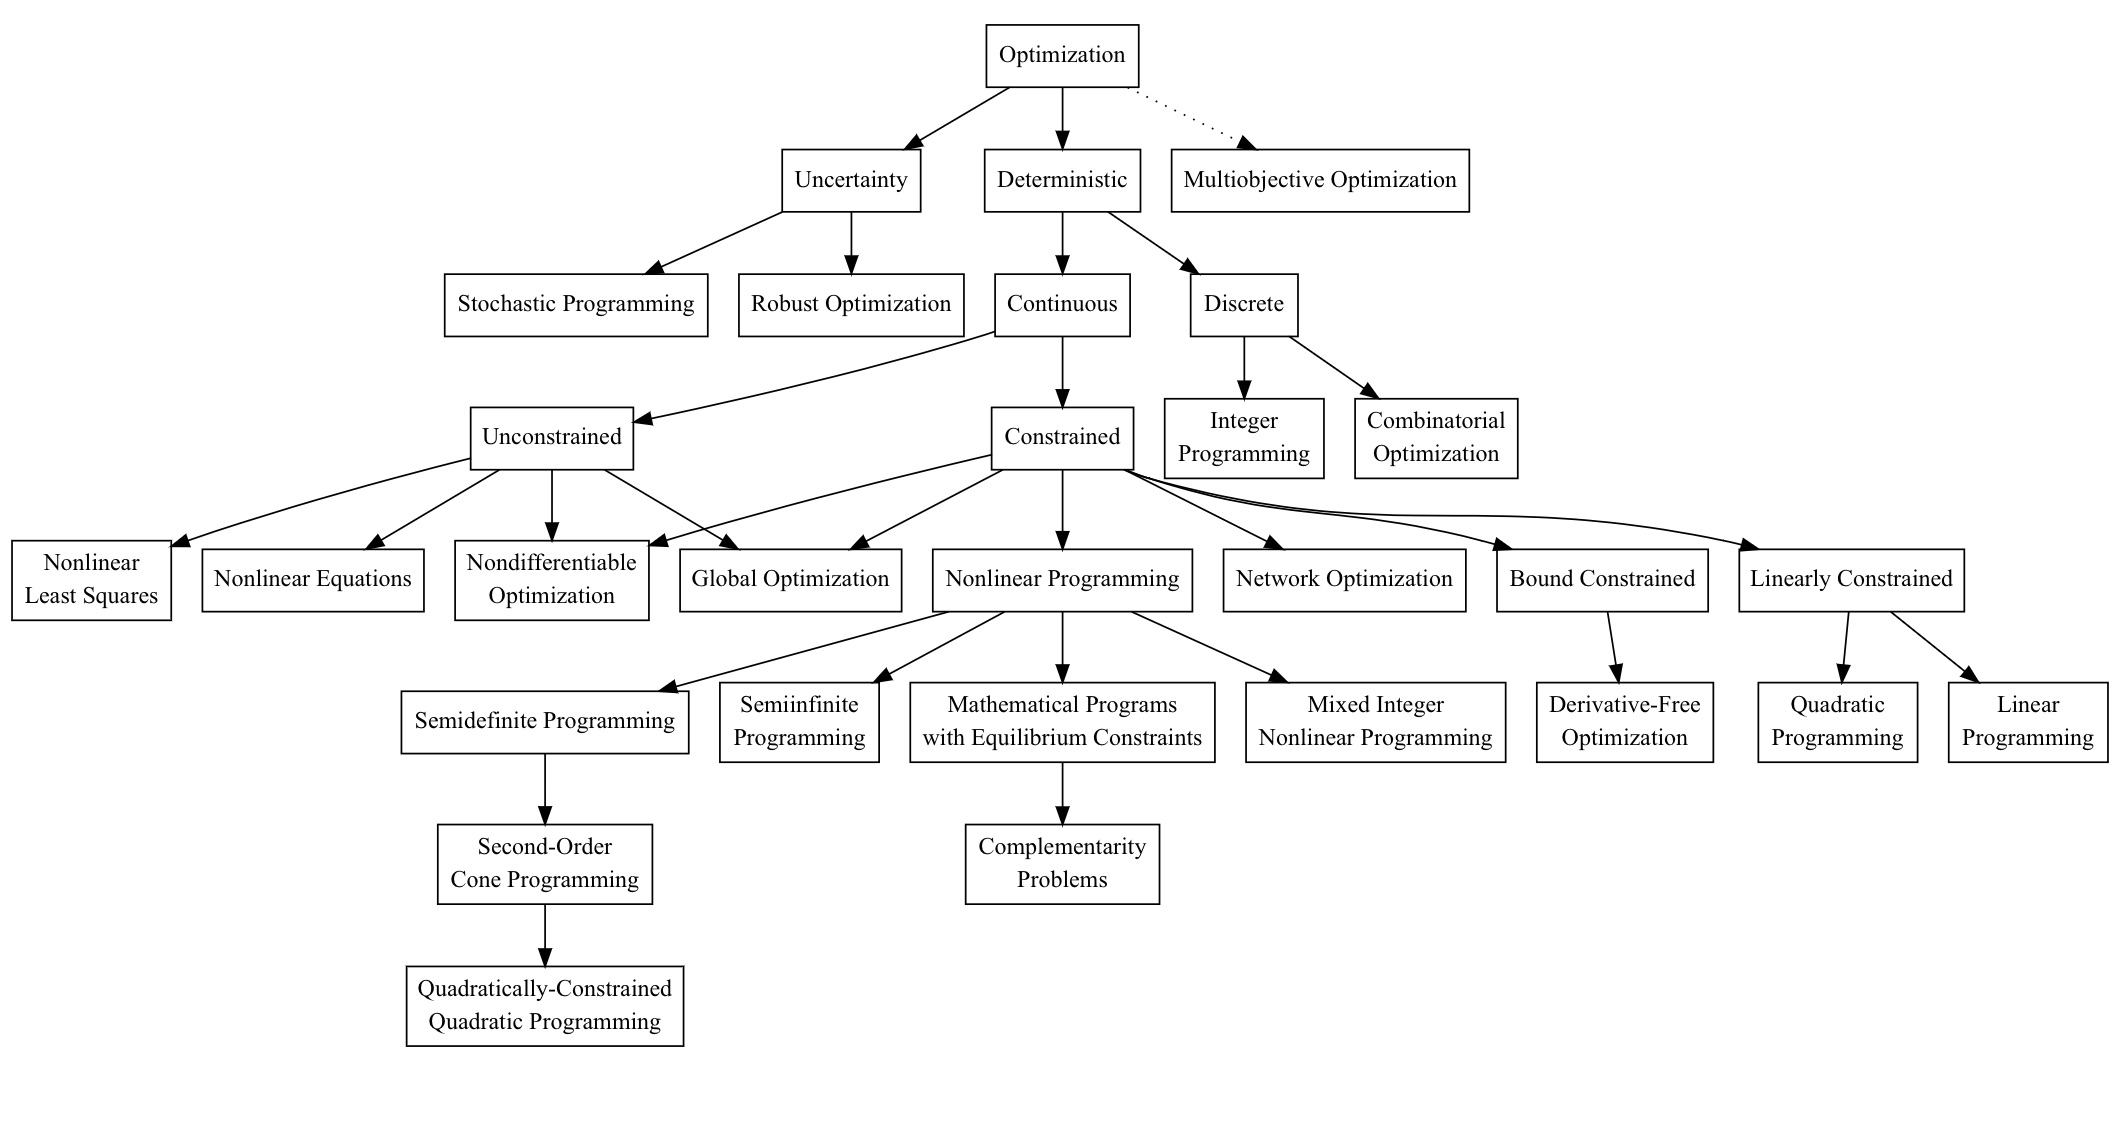
\includegraphics[width=\textwidth]{figs/optimizationtaxonomy.jpeg}
\label{fig:optimizationtaxonomy}
\end{figure}

Moreover, a problem has to meet some more requirements so that it can be written as a QP problem:

\begin{itemize}
    \item The objective function cannot be any function, it needs to be a quadratic function that can be rewritten as follows:
    $$
    f(\mathbf{x}) = \frac{1}{2} \mathbf{x}^{T} \mathbf{Q} \mathbf{x}+\mathbf{c}^{T} \mathbf{x}
    $$
    where $\mathbf{Q}$ is a symmetric $n \times n$ matrix and $\mathbf{c} \in \mathbb{R}^{n \times 1}$.
    \item The constraints must be described by a linear set of equations and inequations:
    $$
    \begin{array}{ll}
        \mathbf{A} \mathbf{x} \leq \mathbf{0}, & \mathbf{A} \in \mathbb{R}^{m \times n} \\
        \mathbf{A_{eq}} \mathbf{x} = \mathbf{0}, & \mathbf{A_{eq}} \in \mathbb{R}^{r \times n}
    \end{array}
    $$
    \item Depending on the characteristics of the matrix $\mathbf{Q}$ the problem can be easily solved using polynomial-time algorithms. This is only posible if $\mathbf{Q}$ positive definite, that is, if all its eigenvalues are greater than or equal to $0$. When $\mathbf{Q}$ is positive definite, the problem is a \textit{convex QP problem}. In the contrary case, the problem is \textit{non-convex} and only local minimums can be found.
\end{itemize}